%!TeX root=MemoriaTFG.tex

\chapter{Resultados}
\label{cap:resultados}

Este capítulo presenta los resultados de la evaluación de modelos
fundacionales dermatológicos y de las contribuciones originales del
trabajo, que concretan sus objetivos formales
(sección~\ref{sec:objetivos}). La secuencia es acumulativa: establecida en la metodología la
independencia entre los conjuntos de evaluación y el preentrenamiento
(sección~\ref{sec:auditoria-resultados}), se estudia la transferencia
supervisada (linear probe, fine-tuning, eficiencia en etiquetas), las
tareas de segmentación,
clasificación \emph{zero-shot} y razonamiento multimodal, y los
aspectos de equidad y seguridad diagnóstica; y, finalmente, las
contribuciones propias sobre DermapixelAI~1.0 y Dermapixel R0, la
interpretabilidad mediante \emph{Sparse Autoencoders} y una síntesis
comparativa. En conjunto, los experimentos permiten analizar el
impacto del preentrenamiento específico de dominio, las distintas
estrategias de adaptación y el papel de los datos en la transferencia
de modelos fundacionales a un entorno clínico dermatológico en
castellano.

\section{Evaluación de PanDerm}
\label{sec:rep-panderm}

El trabajo arranca evaluando PanDerm, el modelo fundacional
dermatológico que se toma como referencia: se mide si sus
representaciones, sin reajustar el encoder, clasifican lesiones
en datasets externos no vistos. El encoder de mayor capacidad
(PanDerm Large) transfiere de forma robusta entre datasets, con
ventaja creciente en los escenarios de mayor heterogeneidad de
adquisición y complejidad taxonómica, como cuantifican los diez
datasets externos a continuación.

La tabla~\ref{tab:lp-panderm} aplica este protocolo a PanDerm Base y
Large sobre los diez datasets externos contrastados, conforme a
sección~\ref{sec:lp}. Se reportan cinco métricas: \emph{accuracy}
(Acc), \emph{balanced accuracy} (BAcc), AUROC \emph{one-vs-rest}, F1
ponderada (W-F1) y coeficiente kappa de Cohen.

\begin{table}[htbp]
\centering
\footnotesize
\setlength{\tabcolsep}{4pt}
\renewcommand{\arraystretch}{0.95}
\caption{Linear probe con PanDerm Base y Large sobre diez datasets
externos. El asterisco (\textsuperscript{$\ast$}) marca Dermnet, el
único dataset con solapamiento exacto frente a Derm1M ($100\%$ por
hash MD5; sección~\ref{sec:auditoria-resultados}).
Mejores valores por dataset y métrica en negrita.}
\label{tab:lp-panderm}
\begin{tabular}{llrrrrr}
\hline
Dataset       & Modelo & Acc            & BAcc           & AUROC          & W-F1           & Kappa \\
\hline
HAM10000      & Base   & $0{,}853$      & $0{,}381$      & $0{,}892$      & $0{,}829$      & $0{,}709$ \\
HAM10000      & Large  & $\mathbf{0{,}888}$ & $\mathbf{0{,}575}$ & $\mathbf{0{,}954}$ & $\mathbf{0{,}880}$ & $\mathbf{0{,}814}$ \\
BCN20000      & Base   & $0{,}659$      & $0{,}292$      & $0{,}855$      & $0{,}615$      & $0{,}447$ \\
BCN20000      & Large  & $\mathbf{0{,}702}$ & $\mathbf{0{,}382}$ & $\mathbf{0{,}903}$ & $\mathbf{0{,}676}$ & $\mathbf{0{,}527}$ \\
PAD-UFES-20   & Base   & $0{,}725$      & $0{,}510$      & $0{,}913$      & $0{,}692$      & $0{,}369$ \\
PAD-UFES-20   & Large  & $\mathbf{0{,}772}$ & $\mathbf{0{,}642}$ & $\mathbf{0{,}949}$ & $\mathbf{0{,}760}$ & $\mathbf{0{,}527}$ \\
Dermnet$^\ast$& Base   & $0{,}450$      & $0{,}381$      & $0{,}888$      & $0{,}432$      & $0{,}437$ \\
Dermnet$^\ast$& Large  & $\mathbf{0{,}550}$ & $\mathbf{0{,}495}$ & $\mathbf{0{,}931}$ & $\mathbf{0{,}540}$ & $\mathbf{0{,}555}$ \\
WSI patches   & Base   & $0{,}781$      & $0{,}640$      & $0{,}976$      & $0{,}774$      & $0{,}842$ \\
WSI patches   & Large  & $\mathbf{0{,}868}$ & $\mathbf{0{,}792}$ & $\mathbf{0{,}991}$ & $\mathbf{0{,}871}$ & $\mathbf{0{,}896}$ \\
DDI           & Base   & $\mathbf{0{,}847}$ & $0{,}714$      & $0{,}827$      & $0{,}836$      & $0{,}482$ \\
DDI           & Large  & $\mathbf{0{,}847}$ & $\mathbf{0{,}764}$ & $\mathbf{0{,}860}$ & $\mathbf{0{,}846}$ & $\mathbf{0{,}535}$ \\
Derm7pt clín. & Base   & $0{,}762$      & $0{,}675$      & $0{,}808$      & $0{,}736$      & $0{,}397$ \\
Derm7pt clín. & Large  & $\mathbf{0{,}798}$ & $\mathbf{0{,}732}$ & $\mathbf{0{,}869}$ & $\mathbf{0{,}784}$ & $\mathbf{0{,}506}$ \\
Derm7pt dermo & Base   & $0{,}818$      & $0{,}749$      & $0{,}841$      & $0{,}811$      & $0{,}528$ \\
Derm7pt dermo & Large  & $\mathbf{0{,}836}$ & $\mathbf{0{,}766}$ & $\mathbf{0{,}858}$ & $\mathbf{0{,}829}$ & $\mathbf{0{,}570}$ \\
HIBA          & Base   & $0{,}883$      & $0{,}595$      & $0{,}894$      & $0{,}853$      & $0{,}275$ \\
HIBA          & Large  & $\mathbf{0{,}904}$ & $\mathbf{0{,}701}$ & $\mathbf{0{,}942}$ & $\mathbf{0{,}892}$ & $\mathbf{0{,}494}$ \\
MSKCC         & Base   & $0{,}721$      & $\mathbf{0{,}654}$ & $0{,}746$      & $0{,}720$      & $0{,}309$ \\
MSKCC         & Large  & $\mathbf{0{,}746}$ & $0{,}644$      & $\mathbf{0{,}751}$ & $\mathbf{0{,}732}$ & $\mathbf{0{,}316}$ \\
\hline
\emph{Media}  & Base   & $0{,}750$      & $0{,}559$      & $0{,}865$      & $0{,}730$      & --- \\
\emph{Media}  & Large  & $\mathbf{0{,}791}$ & $\mathbf{0{,}649}$ & $\mathbf{0{,}901}$ & $\mathbf{0{,}781}$ & --- \\
\hline
\end{tabular}
\end{table}

Sobre los diez datasets evaluados (estimación de semilla única,
sección~\ref{sec:estadistica}), PanDerm Large supera a PanDerm Base en
cuatro de las cinco métricas, con mejoras medias de $+4{,}1$\,pp en
accuracy, $+9{,}0$\,pp en \emph{balanced accuracy} y $+3{,}6$\,pp en
AUROC; la única excepción es la BAcc de MSKCC ($-1{,}0$\,pp;
tabla~\ref{tab:lp-panderm}).

Las mayores ganancias aparecen en Dermnet, WSI~patches y PAD-UFES-20
---los escenarios más heterogéneos del benchmark---, lo que sugiere
que el aumento de capacidad del encoder beneficia especialmente la
generalización compleja. Dermnet, no obstante, está íntegramente
contenido en Derm1M ($100\%$ por hash MD5;
sección~\ref{sec:auditoria-resultados}) y su cifra debe leerse con ese
\emph{caveat}.

En conjunto, los resultados indican que PanDerm mantiene un buen
rendimiento cuando se evalúa sobre datasets distintos del utilizado
para su entrenamiento y en las tres modalidades estudiadas: fotografía
clínica, dermatoscopia e histopatología. La media de todos los datasets
permite resumir la tendencia general, pero no debe interpretarse como
un ranking absoluto entre modelos, ya que cada dataset representa un
problema diferente. Por este motivo, las conclusiones se basan siempre
en el análisis individual de cada uno de ellos
(sección~\ref{sec:agregacion-datasets}).

\section{Comparación con otras familias de modelos}
\label{sec:benchmark}

Para distinguir si la ventaja de PanDerm Large refleja el
preentrenamiento dermatológico o una mera comparación favorable
frente a su versión Base, se sitúa frente a familias con filosofías
de aprendizaje distintas: arquitecturas convolucionales supervisadas,
modelos auto-supervisados generalistas y sistemas vision-language a
gran escala. La tabla~\ref{tab:benchmark} compara cinco modelos
representativos sobre HAM10000, PAD-UFES-20 y DDI bajo el mismo
protocolo de linear probe.

\begin{table}[htbp]
\centering
\footnotesize
\setlength{\tabcolsep}{4pt}
\renewcommand{\arraystretch}{0.95}
\caption{Benchmark comparativo bajo linear probe sobre HAM10000,
PAD-UFES-20 y DDI. Mejor valor por columna en negrita. La AUROC del
DDI de las líneas base convolucionales se calcula sobre $N = 220$
(fusión de validación y test en el \emph{script} de extracción CNN),
frente a $N = 137$ (solo test) en PanDerm~Large y SigLIP; la
convención de promediado de la AUROC multiclase tampoco es homogénea
entre filas (OvR-macro en las CNN, OvR-ponderada en SigLIP, OvO-macro
en PanDerm). Ambas particularidades ---y el mismo desajuste de $N$ en
las filas Gemini de la tabla~\ref{tab:llm-comparativa}--- se
documentan celda a celda en el repositorio reproducible
(\ref{cap:repo}, sección~\ref{sec:repo-bootstrap-ci}).}
\label{tab:benchmark}
\adjustbox{max width=\textwidth}{%
\begin{tabular}{lrrrrrrr}
\hline
Modelo                  & Tipo          & Params & HAM Acc       & HAM AUROC     & PAD Acc       & PAD AUROC     & DDI AUROC \\
\hline
ConvNeXt-Large          & ConvNet sup.  & $197$\,M & $0{,}883$ & $\mathbf{0{,}967}$ & $0{,}668$ & $0{,}894$ & $0{,}774$ \\
EfficientNetV2-Large    & ConvNet sup.  & $118$\,M & $0{,}860$ & $0{,}950$ & $0{,}690$ & $0{,}895$ & $0{,}766$ \\
DINOv2 ViT-L/14         & SSL general   & $307$\,M & $0{,}744$ & $0{,}847$ & ---       & ---       & --- \\
PanDerm Large           & SSL derm.     & $307$\,M & $0{,}888$ & $0{,}954$ & $\mathbf{0{,}772}$ & $\mathbf{0{,}949}$ & $\mathbf{0{,}860}$ \\
SigLIP-Large SO400M     & Vis-leng.\ gen.& $400$\,M & $\mathbf{0{,}900}$ & $0{,}971$ & $0{,}718$ & $0{,}903$ & $0{,}793$ \\
\hline
\end{tabular}}
\end{table}

\begin{figure}[!ht]
\centering

\includegraphics[width=0.88\textwidth]{fig_lp_per_dataset.png}
\caption{Linear probe: AUROC por modelo y dataset sobre los diez
datasets externos. Cinco modelos (DermLIP v2, PanDerm Large, PanDerm
Base, DINOv2 ---evaluado solo en cuatro datasets--- y BiomedCLIP);
``N/A'' indica no evaluado. La celda en rojo, DermLIP v2 sobre Dermnet,
señala el único dataset con solapamiento exacto frente al dataset de
preentrenamiento Derm1M de DermLIP v2
(sección~\ref{sec:auditoria-resultados}); HIBA y MSKCC no presentan
solapamiento.}
\label{fig:lp-per-dataset}
\end{figure}

PanDerm Large supera en accuracy a la mejor CNN supervisada (la mejor
de ConvNeXt-L y EfficientNetV2-L por métrica) sobre los tres
datasets, con ventaja no uniforme: $+0{,}5$\,pp en HAM10000
(dermatoscopia estandarizada) frente a $+8{,}2$\,pp en PAD-UFES-20
(fotografía móvil) y $+2{,}9$\,pp en DDI ($+8{,}6$\,pp AUROC; desglose
en el repositorio reproducible, \ref{cap:repo},
sección~\ref{sec:repo-tablas}).
HAM10000 constituye una excepción parcial: SigLIP-Large SO400M obtiene
la mejor accuracy y AUROC, y ConvNeXt-Large supera ligeramente a
PanDerm Large en AUROC ($-1{,}3$\,pp). Este comportamiento sugiere que
los beneficios del preentrenamiento de dominio son menores en entornos
dermatoscópicos altamente estandarizados; en cambio, PanDerm Large
encabeza en PAD-UFES-20 y DDI, los datasets clínicos más alejados del
dominio web.

La figura~\ref{fig:lp-per-dataset} amplía la comparación a los diez
datasets externos, añadiendo a PanDerm los modelos vision-language
DermLIP v2 y BiomedCLIP y el encoder general DINOv2: ningún modelo
domina en todos los datasets. La única cifra que debe leerse con
cautela es la de DermLIP v2 sobre Dermnet, dataset que forma parte de
su preentrenamiento (Derm1M; sección~\ref{sec:auditoria-resultados}).

No existe, por tanto, una jerarquía universal entre familias: los
sistemas vision-language generalistas igualan o superan a los
especializados en escenarios dermatoscópicos muy estandarizados,
mientras que los modelos dermatológicos mantienen ventaja cuando aumenta
la variabilidad clínica. El preentrenamiento de dominio ofrece una
ventaja \emph{creciente} con la heterogeneidad, no una superioridad
absoluta, lo que anticipa la tesis de especialización por tarea
(sección~\ref{sec:disc-especializacion}). Como modelo dermatológico de
referencia ---abierto y el más sólido sobre los datasets clínicos más
exigentes---, PanDerm se adopta como base de los protocolos que siguen,
en los que se estudia hasta dónde puede llevarse su rendimiento.

\section{Fine-tuning supervisado}
\label{sec:ft-results}

Esta sección delimita cuándo el fine-tuning del encoder mejora sobre
la representación congelada y cuándo es contraproducente, decisión
central para los datasets clínicos pequeños. El fine-tuning mejora con
una cantidad moderada o elevada de datos de entrenamiento y puede
degradar el rendimiento bajo baja disponibilidad de muestras. La
tabla~\ref{tab:ft-panderm} lo concreta comparando el
linear probe con el fine-tuning supervisado de PanDerm Base sobre
cuatro datasets de tamaño dispar, con la configuración descrita
en sección~\ref{sec:ft}. Sobre HAM10000 se añade además
\emph{test-time augmentation} con cinco augmentaciones
deterministas.

\begin{table}[htbp]
\centering
\footnotesize
\setlength{\tabcolsep}{4pt}
\renewcommand{\arraystretch}{0.95}
\caption{Linear probe (LP) frente a fine-tuning (FT) con PanDerm
Base. $\Delta$BAcc en puntos porcentuales respecto al LP.}
\label{tab:ft-panderm}
\begin{tabular}{llrrrrr}
\hline
Dataset      & Modo & Acc           & BAcc          & AUROC         & W-F1          & $\Delta$BAcc \\
\hline
HAM10000     & LP   & $0{,}853$     & $0{,}381$     & $0{,}892$     & $0{,}829$     & --- \\
HAM10000     & FT   & $\mathbf{0{,}920}$ & $\mathbf{0{,}852}$ & $\mathbf{0{,}978}$ & $\mathbf{0{,}923}$ & $+47{,}1$ \\
PAD-UFES-20  & LP   & $0{,}725$     & $0{,}510$     & $0{,}913$     & $0{,}692$     & --- \\
PAD-UFES-20  & FT   & $\mathbf{0{,}755}$ & $\mathbf{0{,}704}$ & $\mathbf{0{,}935}$ & $\mathbf{0{,}757}$ & $+19{,}4$ \\
DDI          & LP   & $\mathbf{0{,}847}$ & $\mathbf{0{,}714}$ & $\mathbf{0{,}827}$ & $\mathbf{0{,}836}$ & --- \\
DDI          & FT   & $0{,}774$     & $0{,}693$     & $0{,}682$     & $0{,}780$     & $-2{,}1$ \\
MSKCC        & LP   & $0{,}721$     & $0{,}654$     & $\mathbf{0{,}746}$ & $0{,}720$     & --- \\
MSKCC        & FT   & $\mathbf{0{,}731}$ & $\mathbf{0{,}684}$ & $0{,}719$     & $\mathbf{0{,}735}$ & $+3{,}0$ \\
\hline
\end{tabular}
\end{table}

El fine-tuning mejora sustancialmente el rendimiento en HAM10000
($+47{,}1$\,pp BAcc) y PAD-UFES-20 ($+19{,}4$\,pp), especialmente
sobre las clases minoritarias responsables de la baja \emph{balanced
accuracy} del linear probe. El beneficio desaparece, en cambio, cuando
disminuye la disponibilidad de datos: DDI muestra degradación global
compatible con sobreajuste y MSKCC sólo mejoras marginales. En la práctica, esto deja una regla sencilla: con un \emph{dataset}
clínico grande conviene hacer fine-tuning, pero con pocos datos
es más seguro quedarse con el encoder congelado, porque el
fine-tuning tiende a sobreajustar. Este resultado justifica la
exploración posterior de adaptación eficiente de parámetros (PEFT,
sección~\ref{sec:dermapixel-spanderm-v0}) y motiva cuantificar cuántas
etiquetas son realmente necesarias, objeto de la sección siguiente.

\section{Eficiencia en etiquetas}
\label{sec:label-eff-results}

Se mide el rendimiento de PanDerm Large bajo submuestreos
estratificados crecientes del conjunto de entrenamiento, dado que el
etiquetado experto es el principal cuello de botella en dermatología.
Una fracción mínima del conjunto basta para casi saturar el
rendimiento. La tabla~\ref{tab:label-eff} lo cuantifica con
submuestreos al $1\%$,
$5\%$, $10\%$, $20\%$, $50\%$ y $100\%$ sobre HAM10000 y
PAD-UFES-20.

\begin{table}[htbp]
\centering
\footnotesize
\setlength{\tabcolsep}{4pt}
\renewcommand{\arraystretch}{0.95}
\caption{Eficiencia en etiquetas (linear probe con PanDerm Large).
$N_{\mathrm{train}}$: tamaño efectivo del subconjunto de
entrenamiento. Mejor valor por columna en negrita.}
\label{tab:label-eff}
\begin{tabular}{lrrrrr}
\hline
$\%$ entrenam.  & $N_{\mathrm{train}}$ & Acc           & BAcc          & AUROC         & W-F1 \\
\hline
\multicolumn{6}{l}{\textit{HAM10000}} \\
$1\%$           & $82$                 & $0{,}850$     & $0{,}406$     & $0{,}918$     & $0{,}828$ \\
$5\%$           & $410$                & $0{,}870$     & $0{,}481$     & $0{,}932$     & $0{,}855$ \\
$10\%$          & $820$                & $0{,}875$     & $0{,}480$     & $0{,}939$     & $0{,}863$ \\
$20\%$          & $1\,641$             & $0{,}882$     & $0{,}547$     & $0{,}951$     & $0{,}873$ \\
$50\%$          & $4\,103$             & $\mathbf{0{,}894}$ & $\mathbf{0{,}589}$ & $0{,}952$ & $\mathbf{0{,}887}$ \\
$100\%$         & $8\,207$             & $0{,}888$     & $0{,}575$     & $\mathbf{0{,}954}$ & $0{,}880$ \\
\hline
\multicolumn{6}{l}{\textit{PAD-UFES-20}} \\
$1\%$           & $14$                 & $0{,}740$     & $0{,}599$     & $0{,}907$     & $0{,}727$ \\
$5\%$           & $74$                 & $0{,}751$     & $0{,}632$     & $0{,}919$     & $0{,}742$ \\
$10\%$          & $149$                & $0{,}738$     & $0{,}593$     & $0{,}923$     & $0{,}724$ \\
$20\%$          & $298$                & $0{,}748$     & $0{,}587$     & $0{,}931$     & $0{,}728$ \\
$50\%$          & $746$                & $0{,}757$     & $0{,}611$     & $0{,}941$     & $0{,}742$ \\
$100\%$         & $1\,493$             & $\mathbf{0{,}772}$ & $\mathbf{0{,}642}$ & $\mathbf{0{,}949}$ & $\mathbf{0{,}760}$ \\
\hline
\end{tabular}
\end{table}

La AUROC satura muy pronto: con el $1\%$ de HAM10000 ($82$ imágenes) ya
alcanza $0{,}918$, y con el $5\%$ ($410$) el $97{,}7\%$ de su máximo; en
PAD-UFES-20 bastan $14$ imágenes para recuperar el $95{,}5\%$ de la
AUROC final. La \emph{balanced accuracy}, en cambio, sigue mejorando
con el volumen, por ser más sensible a las clases minoritarias. Esto
confirma lo anticipado al inicio de la sección: la mayor parte de la
capacidad de discriminar ya está en el encoder preentrenado, y bastan
unas decenas de etiquetas para aprovecharla. Las cifras proceden de una
única partición y semilla por nivel de submuestreo, así que marcan una
tendencia, no un margen con cierre estadístico.

\section{Segmentación binaria de lesión}
\label{sec:seg-results}

Este bloque evalúa si un modelo fundacional de segmentación adaptado
al dominio dermatológico alcanza una delimitación de lesión de calidad
clínica y qué factores la determinan. La tabla~\ref{tab:seg} compara
SAM2.1-Large adaptado al dominio mediante fine-tuning del
decoder frente a SAM2 sin adaptar (\emph{zero-shot}), un
autoencoder convolucional sobre PanDerm Large (CAE-seg) y la
referencia publicada por Yan et~al.~\cite{panderm2025}, analizando
además su generalización fuera de dominio sobre ISIC2017 y PH2; las
subsecciones posteriores aíslan el efecto de la arquitectura, del
\emph{prompt} y de la variabilidad inter-anotador.

\begin{table}[htbp]
\centering
\footnotesize
\setlength{\tabcolsep}{4pt}
\renewcommand{\arraystretch}{0.95}
\caption{Segmentación binaria de lesión: Dice de test sobre tres
datasets dermatoscópicos. Modelos entrenados sobre ISIC2018 y
evaluados sin reentrenamiento sobre ISIC2017 y PH2.}
\label{tab:seg}
\begin{tabular}{lrrr}
\hline
Configuración                         & ISIC2018 Dice & ISIC2017 Dice & PH2 Dice \\
\hline
SAM2 \emph{zero-shot} (bbox de GT)    & ---           & $0{,}797$     & $0{,}886$ \\
CAE-seg (PanDerm-L) FT ISIC2018       & $0{,}894$     & $0{,}879$     & $0{,}924$ \\
PanDerm \cite{panderm2025} (ref.)     & $0{,}921$     & ---           & --- \\
\textbf{SAM2.1-L (decoder FT) ISIC2018}  & $\mathbf{0{,}947}$ & $\mathbf{0{,}945}$ & $\mathbf{0{,}960}$ \\
\hline
\end{tabular}
\end{table}

El detalle con la desviación estándar y el IoU sobre los datasets de
transferencia (ISIC2017 y PH2) figura en el repositorio reproducible
(\ref{cap:repo}, sección~\ref{sec:repo-tablas}).

SAM2.1-L con fine-tuning del decoder alcanza Dice
$0{,}947$ sobre ISIC2018, $+2{,}6$\,pp sobre la cifra publicada por
Yan et~al.~\cite{panderm2025} y $+5{,}3$\,pp sobre el CAE-seg: supera,
por tanto, la referencia previa. Su generalización fuera de dominio es
prácticamente nula (Dice $0{,}945$ en ISIC2017 y $0{,}960$ en PH2,
este último superior por su mayor limpieza visual). Y, sobre todo, la
adaptación del decoder aporta $+14{,}8$\,pp en ISIC2017
($0{,}797 \to 0{,}945$) y $+7{,}4$\,pp en PH2 ($0{,}886 \to 0{,}960$)
frente a SAM2 sin adaptar: es la adaptación al dominio, y no el tamaño
bruto del modelo, lo que explica la mayor parte de la mejora.

Desde una perspectiva aplicada, este resultado anticipa una lectura
que las subsecciones siguientes confirman: una vez disponible una caja
que \emph{localice} la lesión, la calidad del contorno depende poco
del segmentador concreto (sección~\ref{sec:seg-control-automatico}),
de modo que localizar la lesión puede importar más que la precisión
absoluta de la máscara.

\subsection{Comparativa de arquitecturas promptables}
\label{sec:seg-arquitecturas}

La cifra anterior mezcla generación de arquitectura, preentrenamiento
de dominio y tamaño de \emph{backbone}. Para separarlos, se evalúan de
forma pareada cinco arquitecturas \emph{promptables} sobre un dataset
dermatoscópico ampliado y deduplicado por hash MD5 ($14\,201$ imágenes
únicas de ISIC2018, ISIC2017, HAM10000-seg y PH2), bajo régimen común
(fine-tuning denso del decoder y el \emph{promptable
encoder}, encoder visual congelado, \emph{prompt} de \emph{bounding
box} de referencia; detalle de optimización en Cap.~3) y sobre el mismo
test canónico de ISIC2018 ($N = 1\,000$, blindado) que la cifra de
referencia $0{,}947$ de la tabla~\ref{tab:seg}. La
tabla~\ref{tab:seg-arquitecturas} reporta el Dice resultante.

\begin{table}[htbp]
\centering
\footnotesize
\setlength{\tabcolsep}{4pt}
\renewcommand{\arraystretch}{0.95}
\caption{Comparativa de cinco arquitecturas promptables sobre el
test canónico de ISIC2018 ($N = 1\,000$). Régimen común de
fine-tuning del decoder con \emph{prompt} de
\emph{bounding box}. Las diferencias de Dice son modestas en valor
absoluto pero significativas al test de Wilcoxon
pareado~\cite{wilcoxon1945}
($p < 10^{-6}$ en todos los contrastes).}
\label{tab:seg-arquitecturas}
\begin{tabular}{llllrr}
\hline
Modelo            & Arquitectura       & Preentr. & Params & Dice & Latencia \\
\hline
MedSAM2-tiny~\cite{medsam2} & SAM2~\cite{sam2}   & médico   & $39$\,M  & $\mathbf{0{,}9556}$ & $26$\,ms \\
SAM2.1-tiny       & SAM2~\cite{sam2}   & general  & $39$\,M  & $0{,}9517$ & $26$\,ms \\
SAM2.1-Large      & SAM2~\cite{sam2}   & general  & $224$\,M & $0{,}9503$ & $96$\,ms \\
SAM-Med2D~\cite{sammed2d} & SAM~\cite{sam2023} & médico   & $271$\,M & $0{,}9465$ & $20$\,ms \\
MedSAM v1~\cite{medsam}   & SAM~\cite{sam2023} & médico   & $94$\,M  & $0{,}9458$ & $74$\,ms \\
\hline
\end{tabular}
\end{table}

Tres conclusiones emergen de la comparación, con todos los contrastes
pareados significativos (tabla~\ref{tab:seg-arquitecturas}).
\textit{Primero}, la generación
SAM2 aporta más que el preentrenamiento médico: los tres modelos SAM2
superan a los basados en SAM v1, incluso a los de preentrenamiento
médico. \textit{Segundo}, el preentrenamiento médico ofrece una mejora
adicional, pero solo dentro de la misma generación y de menor
magnitud. \textit{Tercero}, el tamaño del \emph{backbone} aporta poco
en régimen \emph{box-prompted}: SAM2.1-tiny iguala o supera a
SAM2.1-Large con $5{,}7$ veces menos parámetros y menor latencia. La
mejor configuración es MedSAM2-tiny ($0{,}9556$, $26$\,ms), que
combina generación SAM2 y preentrenamiento médico en el
\emph{backbone} más compacto. Que la arquitectura pese más que el
preentrenamiento médico matiza la hipótesis central del trabajo: en
este régimen, el diseño del segmentador domina sobre la
especialización dermatológica. Las tres subsecciones siguientes acotan
cuánto del resultado depende del \emph{prompt}, su estabilidad y su
techo real.

La figura~\ref{fig:seg-examples} ilustra estas diferencias de forma
cualitativa: dentro de dominio las tres opciones trazan contornos casi
indistinguibles de la máscara de referencia, y el contraste aparece
fuera de dominio, donde SAM2 sin adaptar puede fallar por completo
mientras que los modelos adaptados se mantienen robustos.

\begin{figure}[p]
\centering
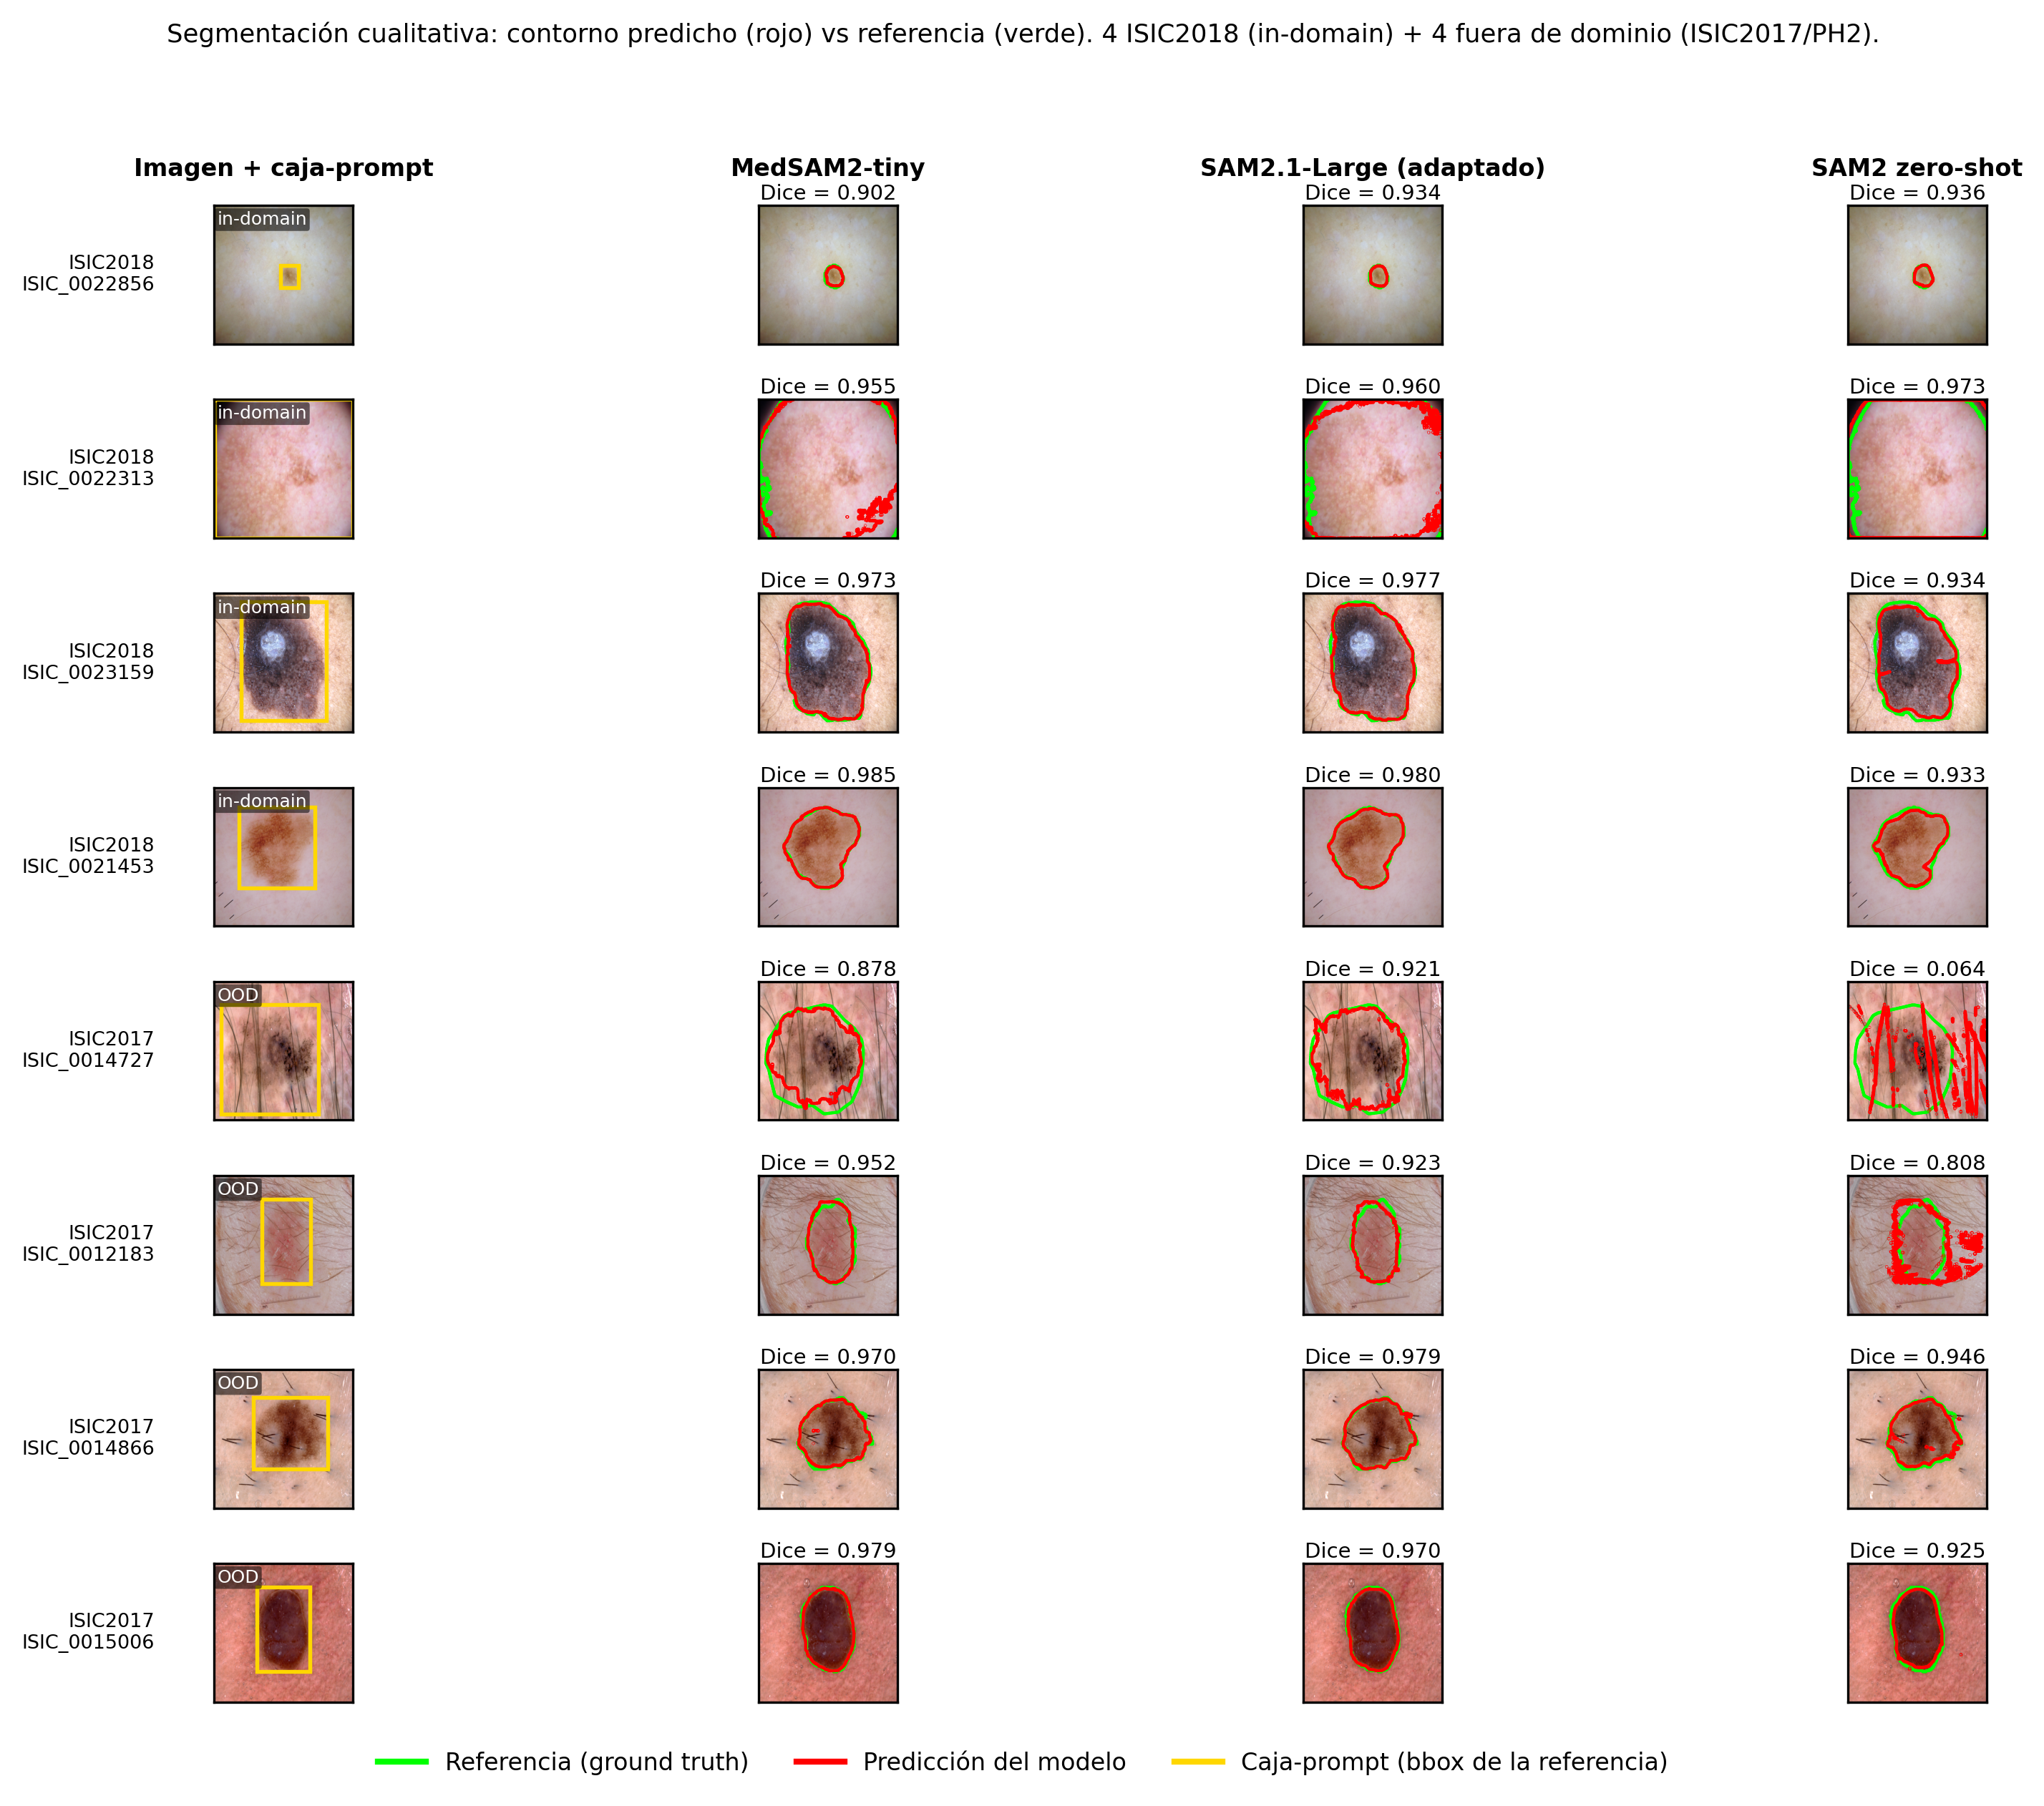
\includegraphics[height=0.85\textheight]{fig_seg_examples.png}
\caption{Ejemplos cualitativos de segmentación sobre ocho lesiones
---cuatro de ISIC2018 (in-domain) y cuatro de ISIC2017 (fuera de
dominio)---. Columna~1: imagen original con la caja-\emph{prompt}
(amarillo) derivada de la máscara de referencia. Columnas~2--4:
MedSAM2-tiny, SAM2.1-Large y SAM2 \emph{zero-shot} (sin adaptar), con
el contorno de referencia (verde) y el predicho (rojo) superpuestos y
el Dice de cada caso. Dentro de dominio las tres opciones se ajustan
bien; fuera de dominio, SAM2 sin adaptar puede colapsar (un caso con
Dice $0{,}064$), mientras que MedSAM2-tiny y SAM2.1-Large permanecen
robustos. Los valores coinciden con el pipeline de evaluación de la
tabla~\ref{tab:seg-arquitecturas}.}
\label{fig:seg-examples}
\end{figure}

\subsection{Valor del prompt: control automático sin caja}
\label{sec:seg-control-automatico}

Toda la comparativa anterior opera en régimen \emph{box-prompted}:
cada predicción parte de una \emph{bounding box} derivada de la
máscara de referencia. Para aislar la contribución de ese
\emph{prompt} se entrena un control automático que no recibe caja
alguna ---una U-Net con encoder ResNet-101 preentrenado en
ImageNet, fine-tuning denso de $51{,}5$\,M de parámetros sobre el
mismo dataset $v1c$--- y se evalúa sobre el test canónico de
ISIC2018, contrastando su Dice con el del mejor modelo
\emph{promptable} (desglose completo con IoU, precisión y recall en el
repositorio reproducible, \ref{cap:repo},
sección~\ref{sec:repo-tablas}).

El control automático alcanza Dice $0{,}8811$, $7{,}5$\,pp por debajo
del mejor modelo \emph{box-prompted} ($0{,}9556$). La comparación de
magnitudes es reveladora: la arquitectura mueve $\sim 1{,}0$\,pp de
Dice (tabla~\ref{tab:seg-arquitecturas}) y el preentrenamiento médico
$\sim 0{,}4$\,pp, pero retirar la caja cuesta $7{,}5$\,pp ---entre
seis y siete veces más que cualquiera de los otros dos factores---. El
factor dominante de la segmentación dermatoscópica no es, por tanto,
ni la arquitectura ni el preentrenamiento, sino la disponibilidad de
una localización razonable de la lesión. El perfil de error del modo automático lo confirma
---recall alto ($0{,}942$) pero precisión desplomada ($0{,}856$) y
Hausdorff~95 entre $2{,}5$ y $3$ veces peor (desv.\ $0{,}121$), señal
de fallos catastróficos puntuales que la caja elimina---. El control
valida además que la comparativa fue justa: todos los modelos
compartían el mismo \emph{prompt}, de modo que sus diferencias
reflejan el segmentador y no la información de localización.

\subsection{Robustez del resultado: validación cruzada, prompt y calibración}
\label{sec:seg-robustez}

La cifra de $0{,}9556$ procede de una única partición. Una validación
cruzada de cinco pliegues sobre MedSAM2-tiny confirma su robustez:
Dice $0{,}9554 \pm 0{,}0010$ (IC95\% $[0{,}9543,\, 0{,}9564]$), con la
cifra principal dentro del intervalo y una desviación inter-pliegue
($8\times 10^{-4}$) que descarta dependencia de una partición
afortunada.

La estabilidad frente a la calidad del \emph{prompt} es crítica en
despliegue, donde la caja procede de un anotador o detector y no de la
máscara de referencia. Bajo perturbaciones controladas, el \emph{jitter}
de esquinas ($\pm 20$ px) apenas resta $0{,}86$\,pp, pero la escala es
crítica y asimétrica: apretar la caja es catastrófico ($-6{,}8$\,pp al
$-10\%$, $-15{,}4$\,pp al $-20\%$, por recortar lesión real) mientras
que aflojarla degrada poco ($-2{,}8$\,pp al $+10\%$;
figura~\ref{fig:seg-box-robustness}). La lectura
operativa se desarrolla en sección~\ref{sec:disc-cv-robustez}.

\begin{figure}[htbp]
\centering

\includegraphics[width=0.82\textwidth]{fig_seg_box_robustness.png}
\caption{Robustez de MedSAM2-tiny a la calidad de la caja-\emph{prompt}
sobre el test canónico de ISIC2018 ($N = 1\,000$). El \emph{jitter}
de esquinas es prácticamente inocuo ($-0{,}86$\,pp), pero la escala
es crítica y asimétrica: apretar la caja degrada mucho más que
aflojarla.}
\label{fig:seg-box-robustness}
\end{figure}

El resto de comprobaciones confirman un modelo bien comportado y no
alteran la conclusión: el ajuste de bajo rango (LoRA
$r\in\{4,8,16,32\}$) iguala al ajuste denso del decoder; la
calibración a nivel de píxel es buena (ECE $0{,}0082$); la equidad por
fototipo (ITA) muestra una brecha de solo $1{,}1$\,pp entre fototipos
extremos; y el aumento en test y el \emph{ensemble} de pliegues aportan
mejoras marginales ($+0{,}13$/$+0{,}14$\,pp) que no compensan su coste,
por lo que se recomienda un único modelo.

\paragraph{Del experimento al prototipo: segmentación automática en
cascada.}
Estos dos hallazgos ---que la caja es lo que más importa y que conviene
que sea holgada--- se aplican tal cual en el prototipo. La U-Net del
control, floja como segmentador por sí sola ($0{,}8811$), es en cambio
un buen \emph{localizador} (recall $0{,}942$), así que se reaprovecha
para \emph{generar} la caja automáticamente. El modo automático
encadena dos pasos: la U-Net localiza la lesión y, del mayor componente
conexo de su máscara, se deriva una \emph{bounding box} a la que se
añade un $10\%$ de margen ---deliberadamente holgada, nunca apretada,
siguiendo el resultado de robustez---; esa caja alimenta a MedSAM2-tiny,
que produce la máscara final (con una caja central de respaldo si la
U-Net no detecta nada). El sistema segmenta así sin intervención
humana, cerrando el bucle del régimen \emph{box-prompted}: la baja
precisión de la U-Net deja de importar, porque su papel no es segmentar,
sino indicar \emph{dónde mirar}. La configuración de la cascada figura
en el repositorio reproducible (\ref{cap:repo},
sección~\ref{sec:repo-prototipo}).

\subsection{El modelo segmenta tan bien como un experto humano}
\label{sec:seg-techo-anotador}

Lo más interesante de este bloque no es el valor absoluto de Dice, sino
compararlo con lo que consigue una persona. El Dice se mide contra una
máscara dibujada a mano, y el borde de una lesión es ambiguo: dos
médicos rara vez trazan exactamente el mismo contorno. Para medir ese
margen humano se empleó el subconjunto de IMA++ con anotación múltiple
($312$ imágenes con dos o más máscaras independientes, reservado y
nunca usado en entrenamiento): dos anotadores humanos coinciden entre
sí solo $0{,}728$, mientras que el modelo coincide con el consenso
$0{,}915$ ---mejor de lo que coinciden los propios médicos--- y queda
dentro de la envolvente de las máscaras humanas el $97{,}8\%$ de las
veces.

De aquí se sigue una consecuencia importante: las diferencias de
$\sim 1$\,pp entre
arquitecturas (tabla~\ref{tab:seg-arquitecturas}) dejan de ser
relevantes ---son más pequeñas que el desacuerdo natural entre dos
personas que dibujan el mismo contorno---: se ha alcanzado el techo de
precisión que la propia tarea permite medir. Conviene acotar esta
conclusión: vale para la segmentación de una sola lesión dermatoscópica
con \emph{prompt} de caja sobre el test blindado de ISIC2018, y no se
extiende a imágenes con varias lesiones ni al uso sin caja. A partir de
aquí, la idea de guiar el modelo con lenguaje ---en lugar de con una
caja--- abre el bloque siguiente, sobre clasificación \emph{zero-shot}
multimodal.

\section{Clasificación zero-shot multimodal}
\label{sec:zs-results}

La clasificación \emph{zero-shot} permite asignar una imagen a un
diagnóstico descrito solo con palabras, sin haber entrenado el modelo
con ejemplos etiquetados de esas categorías. Su interés práctico es
claro: permitiría poner en marcha un sistema sin reunir antes un
\emph{dataset} etiquetado, y añadir diagnósticos nuevos con solo
describirlos. Esta sección estudia de qué depende que ese régimen
funcione, y la respuesta es menos intuitiva de lo esperable: lo
decisivo no es la imagen, sino que el texto y la imagen ``hablen el
mismo idioma'', es decir, que el tokenizer del texto encaje con
el espacio del encoder visual. Se cuantifica sobre HAM10000
($7$ clases, $N_{\mathrm{test}} = 1\,232$) con tres formas de redactar
los \emph{prompts} y dos tokenizers distintos (cifras completas
en el repositorio reproducible, \ref{cap:repo},
sección~\ref{sec:repo-llm}).

El rendimiento depende drásticamente de cómo se construye el texto.
Pasar de \emph{prompts} genéricos en inglés con tokenizer
PubMedBERT al conjunto A3 de Derm1M con tokenizer GPT-2/CLIP eleva
la AUROC de $0{,}366$ a $0{,}854$ ($+48{,}8$\,pp). Los
\emph{prompts} genéricos con PubMedBERT quedan en AUROC$<0{,}5$,
señal de que proyectan en un espacio no alineado con el encoder
visual de la variante v1/v2. Cambiar solo el conjunto A3, sin tocar
el tokenizer, sube la AUROC a $0{,}516$; cambiar solo el
tokenizer, manteniendo A3, la lleva a $0{,}854$. El principal cuello
de botella del régimen \emph{zero-shot} no reside, por tanto, en la
representación visual ---idéntica en todas las configuraciones---,
sino en la alineación entre el espacio textual y el espacio visual.

Esta diferencia de casi $50$\,pp de AUROC, obtenida sin modificar el
encoder visual ni las imágenes, tiene una implicación metodológica
directa: evaluar un modelo \emph{zero-shot} con una única configuración
de \emph{prompts} o tokenizers puede falsear sus capacidades
reales, y una comparación entre modelos puede incluso invertirse según
el \emph{prompt} elegido.

La generalización de este comportamiento a escenarios clínicos
externos se evalúa sobre la tarea binaria melanoma/no-melanoma en
cuatro datasets independientes
(DDI, MSKCC, HIBA y Derm7pt clínico) con la configuración
PubMedBERT de DermLIP v1/v2 (cifras por dataset en el repositorio
reproducible, \ref{cap:repo}, sección~\ref{sec:repo-tablas}).

La sensibilidad observada en HAM10000 se reproduce en los cuatro
datasets externos: bajo la configuración PubMedBERT con \emph{prompts}
genéricos, DermLIP opera cerca del azar (BAcc $\approx 0{,}5$ sobre
DDI, MSKCC, HIBA y Derm7pt clínico), lo que
confirma que el rendimiento \emph{zero-shot} depende críticamente de la
alineación texto-imagen y limita la robustez del paradigma zero-shot
puro (análisis extendido en el repositorio reproducible, \ref{cap:repo}, sección~\ref{sec:repo-llm}).

\paragraph{El idioma del espacio latente: una exploración en el
prototipo.}
Conviene detenerse aquí, porque es una de las ideas que más ilusión
despiertan. Un modelo como DermLIP coloca imágenes y textos en un mismo
``mapa'' ---un espacio latente compartido---, y clasificar en
\emph{zero-shot} no es más que mirar qué etiqueta de texto cae más
cerca de la imagen. Eso es muy potente ---se añade un diagnóstico nuevo
con solo escribir su nombre--- pero también frágil: si la frase no
aterriza en el sitio correcto del mapa, el modelo falla aunque la
lesión sea perfectamente reconocible.

Y ahí entra un eje decisivo para un sistema en castellano: el idioma.
El codificador de texto de estos modelos se entrenó casi todo en
inglés, de modo que su mapa está ``anclado'' al inglés y el español
crudo cae en una zona peor alineada. En el prototipo se está explorando
exactamente esto ---describir los conceptos en español, en inglés, o en
español traducido al inglés antes de codificarlos---. El efecto es
llamativo: en un caso real de carcinoma basocelular, con las etiquetas
en español el modelo lo situaba por detrás del melanoma; traduciendo
esas mismas etiquetas al inglés ---misma imagen, mismo modelo, solo
cambian las palabras--- pasaba a reconocer el carcinoma basocelular con
clara ventaja. No se reentrena nada: se trata de ``hablarle'' al modelo
en el idioma de su espacio latente. Estas confianzas son relativas
entre las opciones, no diagnósticos calibrados, y la exploración sigue
en curso; pero ya marca el camino ---un glosario clínico
español$\to$inglés a corto plazo y, a más largo, un modelo realmente
alineado con el español, la misma motivación que la rama contrastiva
castellana de Dermapixel~R0 (sección~\ref{sec:spanderm-clip})---.

\section{Comparación con modelos generativos generalistas}
\label{sec:llm-results}

Esta sección contrasta si los grandes modelos de lenguaje
multimodales, entrenados sobre datasets mucho mayores, cierran la
brecha frente a los especialistas. La
tabla~\ref{tab:llm-comparativa} evalúa seis modelos de lenguaje
multimodales sobre HAM10000, PAD-UFES-20 y DDI, junto a los modelos de
referencia de las secciones~\ref{sec:rep-panderm}
y~\ref{sec:ft-results}.

\begin{table}[htbp]
\centering
\footnotesize
\setlength{\tabcolsep}{4pt}
\renewcommand{\arraystretch}{0.95}
\caption{Comparación de paradigmas sobre HAM10000, PAD-UFES-20 y DDI
($N_{\mathrm{test}} = 1\,232 / 461 / 137$). FT: fine-tuning, LP:
linear probe, ZS: zero-shot.}
\label{tab:llm-comparativa}
\begin{tabular}{llrrrrrr}
\hline
Modelo                 & Modo  & HAM Acc       & HAM BAcc      & PAD Acc       & PAD BAcc      & DDI Acc       & DDI BAcc \\
\hline
PanDerm Base (TTA HAM) & FT    & $\mathbf{0{,}920}$ & $\mathbf{0{,}852}$ & $0{,}755$     & $\mathbf{0{,}704}$ & $0{,}774$     & $0{,}693$ \\
PanDerm Large          & LP    & $0{,}888$     & $0{,}575$     & $\mathbf{0{,}772}$ & $0{,}642$     & $\mathbf{0{,}847}$ & $\mathbf{0{,}764}$ \\
SigLIP-Large           & LP    & $0{,}900$     & ---           & $0{,}718$     & ---           & $0{,}789$     & --- \\
MedGemma 27B + LoRA    & FT    & $0{,}802$     & $0{,}270$     & $0{,}430$     & $0{,}347$     & $0{,}657$     & $0{,}618$ \\
MedGemma 27B           & ZS    & $0{,}665$     & $0{,}243$     & $0{,}447$     & $0{,}342$     & $0{,}474$     & $0{,}566$ \\
GPT-4o                 & ZS    & $0{,}485$     & $0{,}465$     & $0{,}553$     & $0{,}523$     & $0{,}723$     & $0{,}648$ \\
GPT-4o-mini            & ZS    & $0{,}256$     & $0{,}319$     & $0{,}390$     & $0{,}435$     & $0{,}737$     & $0{,}556$ \\
Gemini 2.5 Pro         & ZS    & $0{,}403$     & ---           & $0{,}477$     & ---           & $0{,}441$     & --- \\
Gemini 2.5 Flash       & ZS    & $0{,}380$     & ---           & $0{,}486$     & ---           & $0{,}555$     & --- \\
DermLIP                & ZS    & $0{,}239$     & $0{,}581$     & $0{,}601$     & ---           & $0{,}329$     & --- \\
BLIP-2 (Flan-T5-XL)    & ZS    & $0{,}015$     & $0{,}145$     & $0{,}017$     & $0{,}167$     & $0{,}796$     & $0{,}542$ \\
InstructBLIP (Flan-T5-XL)& ZS  & $0{,}024$     & $0{,}123$     & $0{,}171$     & $0{,}224$     & $0{,}788$     & $0{,}500$ \\
\hline
\end{tabular}
\end{table}

Los resultados separan claramente especialistas y generalistas. El
mejor sistema dermatológico (PanDerm Base ajustado con TTA) alcanza
accuracy $0{,}920$ sobre HAM10000, frente a $0{,}485$ del mejor
generalista \emph{zero-shot} (GPT-4o) ---una diferencia de $43{,}5$\,pp
(figura~\ref{fig:llm-comparison}) que se mantiene en PAD-UFES-20 y DDI---; en el extremo inferior, BLIP-2 e
InstructBLIP caen a accuracy $\sim 0{,}02$ sobre HAM10000. La lectura
no es que un modelo generalista sea deficiente, sino que, cuando el
problema es extremadamente visual y especializado, el conocimiento
dermatológico adquirido durante el preentrenamiento domina sobre la
mayor capacidad lingüística de los modelos multimodales
generalistas.\footnote{Las cifras de los modelos accesibles por API
comercial corresponden al \emph{prompt} y a la versión del proveedor
disponibles en la fecha de evaluación, no reproducible ante
actualizaciones silenciosas (sección~\ref{sec:lim-pesos}); documentan
un punto de comparación reproducible en su formulación, no el techo
intrínseco de cada sistema.}

\begin{figure}[htbp]
\centering

\includegraphics[width=0.92\textwidth]{fig_llm_comparison.png}
\caption{Comparativa de paradigmas sobre HAM10000. Gradiente
de $43{,}5$\,pp accuracy entre el mejor especialista
ajustado (PanDerm Base FT con TTA, $0{,}920$) y el mejor LLM
multimodal generalista \emph{zero-shot} (GPT-4o,
$0{,}485$). BLIP-2 e InstructBLIP descienden hasta accuracy
$\sim 0{,}02$.}
\label{fig:llm-comparison}
\end{figure}

\subsection{Ajuste supervisado de un LLM multimodal: MedGemma con LoRA}

MedGemma es el único LLM multimodal que se acerca, y lo hace gracias a
la adaptación al dominio: el ajuste con LoRA sobre MedGemma~27B mejora
$+13{,}7$\,pp de accuracy sobre HAM10000 respecto a su variante
\emph{zero-shot} ($0{,}665 \to 0{,}802$) ---un salto que vuelve a
señalar que es la adaptación, y no la escala bruta, lo que cierra la
brecha---. Aun así, incluso adaptado queda $11{,}8$\,pp por debajo del
mejor especialista y la mejora no transfiere de forma sistemática
(sin ganancia sobre PAD-UFES-20). El desglose por dataset, los
patrones de error de GPT-4o y los costes de inferencia figuran en el
repositorio reproducible (\ref{cap:repo}, sección~\ref{sec:repo-llm}).

\section{Equidad por fototipo cutáneo}
\label{sec:equidad-results}

Esta sección analiza si los modelos rinden de forma equitativa entre
fototipos cutáneos y cómo distinguir una equidad real de una métrica
engañosa: un \emph{gap} pequeño puede esconder un modelo
uniformemente peor, de modo que la métrica aislada no decide, como
establecen la comparación de cinco encoders y el test de DeLong. El rendimiento global de los cinco encoders sobre Fitzpatrick17k
completo ($N = 16\,577$), en las dos formulaciones consideradas
---$114$ patologías y $3$ clases de malignidad---, figura en el
repositorio reproducible (\ref{cap:repo}, sección~\ref{sec:repo-tablas}); el análisis
de equidad se centra en la formulación de $3$ clases. La
tabla~\ref{tab:equidad-fototipo} reporta la BAcc por fototipo
Fitzpatrick sobre esa formulación.

\begin{table}[htbp]
\centering
\footnotesize
\setlength{\tabcolsep}{4pt}
\renewcommand{\arraystretch}{0.95}
\caption{BAcc por subgrupo Fitzpatrick (3 clases de malignidad) y
\emph{gap} entre fototipos extremos. Tamaños muestrales por
subgrupo: $299 / 470 / 325 / 261 / 169 / 73$ para FST~I a~VI.}
\label{tab:equidad-fototipo}
\begin{tabular}{lrrrrrrr}
\hline
Modelo                    & FST I         & FST II        & FST III       & FST IV        & FST V         & FST VI        & Gap I-VI \\
\hline
PanDerm Large             & $0{,}723$     & $0{,}708$     & $0{,}743$     & $0{,}669$     & $0{,}568$     & $0{,}506$     & $+0{,}217$ \\
PanDerm Base              & $0{,}653$     & $0{,}693$     & $0{,}669$     & $0{,}630$     & $0{,}585$     & $0{,}384$     & $+0{,}269$ \\
DermLIP v2 (visual)       & $0{,}716$     & $0{,}730$     & $0{,}765$     & $0{,}710$     & $0{,}693$     & $0{,}434$     & $+0{,}281$ \\
DINOv2 ViT-L/14           & $0{,}673$     & $0{,}671$     & $0{,}679$     & $0{,}654$     & $0{,}553$     & $0{,}368$     & $+0{,}306$ \\
BiomedCLIP                & $0{,}569$     & $0{,}602$     & $0{,}606$     & $0{,}566$     & $0{,}590$     & $\mathbf{0{,}445}$ & $\mathbf{+0{,}124}$ \\
\hline
\end{tabular}
\end{table}

Los cinco modelos tienen \emph{gap}~I-VI positivo
(figura~\ref{fig:fairness-5models}): todos rinden peor
sobre los fototipos elevados. Pero el ranking de equidad no coincide
con el de rendimiento. DermLIP v2
logra la mejor BAcc global ($0{,}721$ sobre $3$ clases) y la mejor
AUROC ($0{,}909$), pero con un \emph{gap}~I-VI ($+0{,}281$) mayor que
el de PanDerm Large ($+0{,}217$); y BiomedCLIP exhibe el \emph{gap}
menor ($+0{,}124$) pero la peor BAcc global ($0{,}590$).

\begin{figure}[htbp]
\centering

\includegraphics[width=0.95\textwidth]{figura_fairness_5models.png}
\caption{Equidad por fototipo Fitzpatrick (formulación de tres
clases de malignidad) sobre los cinco encoders evaluados. Los
cinco presentan \emph{gap}~I-VI positivo (entre $+0{,}124$ y
$+0{,}306$\,pp BAcc). Paradoja BiomedCLIP: \emph{gap} mínimo
asociado a peor BAcc global, lo que demuestra el carácter no
decisional de la métrica aislada.}
\label{fig:fairness-5models}
\end{figure}

Este contraste encierra la principal aportación metodológica de la
sección: \textbf{el \emph{gap} aislado no constituye una métrica
suficiente de equidad}. Un modelo uniformemente peor entre subgrupos
puede presentar una brecha reducida simplemente porque falla en todos
ellos ---ser equitativamente malo no es ser equitativo en sentido
sustantivo---. La interpretación debe además acotarse por el reducido
tamaño muestral del fototipo~VI ($N = 73$, frente a $299$ en
FST~I; sección~\ref{sec:lim-muestrales}), que ensancha los intervalos
del \emph{gap} sobre los fototipos oscuros (tabla~\ref{tab:equidad-gap-ci}).
El contraste con cierre estadístico se reserva al test de DeLong
(sección~\ref{sec:equidad-delong}).

\begin{table}[htbp]
\centering
\footnotesize
\caption{\emph{Gap} de equidad I-VI (BAcc FST~I $-$ BAcc FST~VI) con
intervalo de confianza al $95\%$ por \emph{bootstrap} ($B = 1\,000$,
estratificado). El reducido tamaño de FST~VI ($N = 73$) ensancha los
intervalos; el de BiomedCLIP incluye el cero, de modo que su
\emph{gap} mínimo no es estadísticamente distinguible de la ausencia
de disparidad. Intervalos por subgrupo en el repositorio reproducible
(\ref{cap:repo}, sección~\ref{sec:repo-bootstrap-ci}).}
\label{tab:equidad-gap-ci}
\begin{tabular}{lc}
\hline
Modelo & \emph{Gap}~I-VI $[$IC$\,95\%]$ \\
\hline
PanDerm Large   & $0{,}217$ $[0{,}015,\, 0{,}387]$ \\
PanDerm Base    & $0{,}269$ $[0{,}116,\, 0{,}389]$ \\
DermLIP v2      & $0{,}281$ $[0{,}109,\, 0{,}430]$ \\
DINOv2 ViT-L/14 & $0{,}306$ $[0{,}136,\, 0{,}426]$ \\
BiomedCLIP      & $0{,}124$ $[-0{,}052,\, 0{,}280]$ \\
\hline
\end{tabular}
\end{table}

Un experimento cruzado \emph{Light}~$\leftrightarrow$~\emph{Dark}
(\emph{Light} agrupa FST~I-III; \emph{Dark}, FST~IV-VI; matriz completa
en el repositorio reproducible, \ref{cap:repo}, sección~\ref{sec:repo-tablas}) añade una
segunda lectura, más fuerte que el simple \emph{gap}.
Entrenar solo con fototipos claros y evaluar sobre oscuros (L$\to$D
frente a L$\to$L) penaliza el rendimiento. La caída es mayor en
DINOv2 ($\Delta = -0{,}132$\,pp BAcc) y menor en BiomedCLIP
($\Delta = -0{,}063$\,pp). DermLIP v2 muestra la menor caída
Dark$\to$Light frente a Dark$\to$Dark ($\Delta = +0{,}016$\,pp), lo
que apunta a representaciones más invariantes al fototipo cutáneo.

La proximidad entre algunos resultados ---especialmente entre PanDerm
Large y DermLIP v2--- plantea si las diferencias reflejan una ventaja
real o son compatibles con la variabilidad muestral, lo que motiva un
contraste formal mediante el test de DeLong.

\subsection{Validación estadística del ranking de encoders: test de
DeLong}
\label{sec:equidad-delong}

El contraste estadístico formal mediante el test de
DeLong~\cite{delong1988} ---que controla la correlación de evaluar
varios modelos sobre las mismas imágenes--- se aplica a tres
\emph{endpoints} binarios centrales de detección de lesión maligna:
malignidad sobre Fitzpatrick17k, melanoma sobre HAM10000 y malignidad
sobre DermapixelAI~1.0. En cada uno, la comparación entre modelos parte
de una regresión logística binaria sobre sus \emph{features} congeladas
(sección~\ref{sec:lp}) y los $p$-valores pareados se corrigen por el
método de Holm dentro del \emph{endpoint}. Las comparaciones se
interpretan como contrastes centrales del estudio.

\paragraph{Endpoint 1: malignidad sobre Fitzpatrick17k.}
Sobre el test de Fitzpatrick17k ($N = 1\,658$, $226$ malignos), la
tabla~\ref{tab:delong-auroc} reporta la AUROC binaria con IC95\% por la
varianza de DeLong; la matriz completa de $p$-valores pareados (dos
colas) figura en el repositorio reproducible (\ref{cap:repo},
sección~\ref{sec:repo-tablas}).

\begin{table}[htbp]
\centering
\footnotesize
\setlength{\tabcolsep}{4pt}
\renewcommand{\arraystretch}{0.95}
\caption{AUROC binaria de detección de malignidad (\emph{maligno}
frente al resto) sobre el test de Fitzpatrick17k
($N = 1\,658$, $226$ malignos), con intervalo de confianza al
$95\%$ por la varianza de DeLong. Mejor valor en negrita.}
\label{tab:delong-auroc}
\begin{tabular}{lrl}
\hline
Modelo            & AUROC               & IC95\% (DeLong) \\
\hline
PanDerm Large     & $\mathbf{0{,}9488}$ & $[0{,}9350,\, 0{,}9626]$ \\
DermLIP v2        & $0{,}9452$          & $[0{,}9307,\, 0{,}9598]$ \\
PanDerm Base      & $0{,}9296$          & $[0{,}9130,\, 0{,}9463]$ \\
DINOv2 ViT-L/14   & $0{,}9150$          & $[0{,}8932,\, 0{,}9367]$ \\
BiomedCLIP        & $0{,}8915$          & $[0{,}8672,\, 0{,}9158]$ \\
\hline
\end{tabular}
\end{table}

El test de DeLong confirma que PanDerm Large y DermLIP v2 presentan un
rendimiento estadísticamente indistinguible
($\Delta\mathrm{AUROC} = 0{,}0036$, $p = 0{,}55$): ningún dato sostiene
una jerarquía entre ambos sobre este \emph{endpoint}. Los dos superan,
en cambio, de forma significativa a los encoders generalistas (DINOv2
y BiomedCLIP) y a PanDerm Base ($p \leq 7{,}3\times 10^{-3}$ en los
seis contrastes), lo que respalda cuantitativamente la ventaja del
preentrenamiento específico de dominio. Tras la corrección de Holm,
siete de los diez contrastes se mantienen significativos, mientras que
algunas comparaciones entre generalistas (DINOv2--BiomedCLIP,
DINOv2--PanDerm~Base) dejan de ser concluyentes, delimitando qué
distinciones del \emph{ranking} son señal y cuáles ruido muestral.

\paragraph{Endpoint 2: melanoma sobre HAM10000.}
El mismo contraste se aplica al \emph{endpoint} binario melanoma frente
al resto sobre el test de HAM10000 ($N = 1\,232$, $70$ melanomas),
incorporando SigLIP-Large al conjunto de encoders con AUROC
publicada sobre este dataset. La tabla~\ref{tab:delong-ham} reporta las
cifras.

\begin{table}[htbp]
\centering
\footnotesize
\setlength{\tabcolsep}{4pt}
\renewcommand{\arraystretch}{0.95}
\caption{AUROC binaria de detección de melanoma (\emph{melanoma} frente
al resto) sobre el test de HAM10000 ($N = 1\,232$, $70$ melanomas), con
intervalo de confianza al $95\%$ por la varianza de DeLong. Ningún
contraste pareado resulta significativo tras la corrección de Holm
($p_{\mathrm{Holm}} = 1{,}0$ en los tres). Mejor valor en negrita.}
\label{tab:delong-ham}
\begin{tabular}{lrl}
\hline
Modelo          & AUROC               & IC95\% (DeLong) \\
\hline
PanDerm Large   & $\mathbf{0{,}9523}$ & $[0{,}9314,\, 0{,}9733]$ \\
SigLIP-Large    & $0{,}9495$          & $[0{,}9245,\, 0{,}9745]$ \\
DermLIP v2      & $0{,}9463$          & $[0{,}9246,\, 0{,}9681]$ \\
\hline
\end{tabular}
\end{table}

Los tres encoders alcanzan AUROC en torno a $0{,}95$ con
diferencias inferiores a $0{,}006$, y ningún contraste pareado resulta
significativo tras la corrección de Holm (todos con $p_{\mathrm{Holm}} =
1{,}0$): sobre este \emph{endpoint}, PanDerm Large, SigLIP-Large y
DermLIP v2 son estadísticamente indistinguibles. Con sólo $70$
positivos, la potencia es insuficiente para separar modelos cuyas AUROC
se solapan ampliamente.

Sobre este mismo \emph{endpoint}, la discriminación es fuerte
(AUROC $\sim 0{,}95$) \emph{y} la calibración de las probabilidades
resulta razonable: reutilizando las mismas predicciones por muestra
del contraste de DeLong (head de regresión logística \emph{train}$\to$\emph{test},
sin reentrenamiento), el error de calibración esperado
(ECE, $15$ \emph{bins} de igual anchura sobre la probabilidad de la
clase positiva) y el \emph{Brier score} son de
ECE${}=0{,}017$ y \emph{Brier}${}=0{,}029$ para PanDerm Large,
ECE${}=0{,}017$ y \emph{Brier}${}=0{,}030$ para SigLIP-Large, y
ECE${}=0{,}018$ y \emph{Brier}${}=0{,}031$ para DermLIP v2 (curvas de
fiabilidad por \emph{bin} en el repositorio reproducible,
\ref{cap:repo}, sección~\ref{sec:repo-calibracion-ham}). El análisis
sistemático de calibración entre tareas queda fuera del alcance de este
trabajo (capítulo~\ref{cap:limitaciones}, sección de elementos no
abordados).

\paragraph{Endpoint 3: malignidad sobre DermapixelAI~1.0 (protocolo
distinto).} El tercer \emph{endpoint} ---malignidad frente al resto
sobre DermapixelAI~1.0--- requiere una salvedad de protocolo. El
\emph{split} de test canónico (sección~\ref{sec:dermapixel-results}) es
de tamaño limitado para inferencia binaria ($N = 36$, sólo $3$
positivos), por lo que el contraste de DeLong se estima en su lugar
mediante una validación cruzada de cinco pliegues
\emph{out-of-fold} sobre el dataset completo ($N = 1\,062$, $58$
malignos; tabla~\ref{tab:delong-dermapixel}), con DeLong pareado sobre
las predicciones agrupadas y corrección de Holm. Este protocolo difiere del de los dos
\emph{endpoints} anteriores (train$\to$test) y se emplea por el
tamaño limitado del \emph{split} fijo.

\begin{table}[htbp]
\centering
\footnotesize
\setlength{\tabcolsep}{4pt}
\renewcommand{\arraystretch}{0.95}
\caption{AUROC binaria de detección de malignidad sobre DermapixelAI~1.0
estimada por validación cruzada \emph{out-of-fold} de cinco pliegues
($N = 1\,062$, $58$ malignos), con intervalo de confianza al $95\%$ por
la varianza de DeLong. Protocolo distinto del de los \emph{endpoints}
train$\to$test por el tamaño limitado del \emph{split} fijo. Ningún
contraste pareado alcanza significación tras la corrección de Holm.
Mejor valor en negrita.}
\label{tab:delong-dermapixel}
\begin{tabular}{lrl}
\hline
Modelo          & AUROC (OOF)         & IC95\% (DeLong) \\
\hline
DermLIP v2      & $\mathbf{0{,}8946}$ & $[0{,}8472,\, 0{,}9421]$ \\
PanDerm Large   & $0{,}8632$          & $[0{,}8075,\, 0{,}9189]$ \\
PanDerm Base    & $0{,}8630$          & $[0{,}8097,\, 0{,}9163]$ \\
CLIP-L          & $0{,}8536$          & $[0{,}7926,\, 0{,}9146]$ \\
DINOv2          & $0{,}8469$          & $[0{,}7980,\, 0{,}8958]$ \\
\hline
\end{tabular}
\end{table}

DermLIP v2 obtiene el mejor valor puntual (AUROC $= 0{,}8946$), por
delante de PanDerm Large ($0{,}8632$) y del resto ($0{,}85$--$0{,}86$),
pero ningún par de contrastes alcanza significación tras la corrección
de Holm: con $58$ positivos el \emph{endpoint} no tiene potencia para
ordenar los modelos. Dermapixel R0 queda fuera de este contraste, cuyo
alcance se circunscribe a los encoders congelados.

En conjunto, el cierre estadístico se concentra en Fitzpatrick17k ---el
único \emph{endpoint} con potencia suficiente ($226$ positivos)---,
donde la jerarquía «específico de dominio $>$ generalista» es
significativa sin sostener una ordenación fina entre los dos líderes
específicos. Los \emph{endpoints} de HAM10000 ($70$ melanomas) y
DermapixelAI~1.0 ($58$ malignos) corroboran de forma descriptiva ese
patrón ---AUROC elevadas y solapadas--- sin alcanzar significación, un
resultado compatible con la falta de potencia y no con la ausencia de
efecto. La lectura que habilita el contraste es, por tanto, más sólida
que coronar a un único modelo: los resultados no identifican un encoder
dermatológico claramente superior, sino una \emph{familia} de encoders
dermatológicos que supera de forma consistente a los modelos
generalistas, conclusión que se retoma en la discusión
(sección~\ref{sec:disc-especializacion}).

\section{Interpretabilidad del SAE: alineamiento con conceptos
dermatoscópicos clásicos}
\label{sec:sae-derm7pt}

De todas las ideas exploradas en este trabajo, esta es la que más
ilusión despierta de cara a la consulta: para que un dermatólogo
confíe en una IA no basta con que acierte, necesita saber \emph{por
qué} lo dice. La pregunta de esta sección es si el modelo, por dentro,
``razona'' con los mismos conceptos que usa un especialista al mirar
una dermatoscopia ---retículo pigmentado, glóbulos, velo
azul-blanquecino, vasos--- o si es una caja negra.

La herramienta para averiguarlo es un \emph{Sparse Autoencoder} (SAE):
una red auxiliar que toma la representación interna de PanDerm ---un
vector denso y opaco--- y la descompone en un diccionario de $16\,384$
\emph{features} dispersas, cada una idealmente asociada a un patrón
visual concreto. Se entrenó sobre las activaciones de PanDerm Large y
se contrastó contra dos vocabularios de conceptos ya anotados por
dermatólogos: los $48$ de SkinCon~\cite{skincon} y los siete criterios
del \emph{Seven-Point Checklist} de Derm7pt~\cite{kawahara2019}
($1\,011$ lesiones dermatoscópicas, \emph{splits} oficiales
$413$/$203$/$395$, $24{,}5\%$ melanomas). El detalle del entrenamiento
del SAE figura en el repositorio reproducible (\ref{cap:repo},
sección~\ref{sec:repo-sae}).

\paragraph{¿El modelo ya ``ve'' los conceptos del dermatólogo?}
La respuesta es que sí, y sin que nadie se lo enseñara. Tomando cada
una de las $16\,384$ \emph{features} como un posible detector de cada
criterio, las mejores distinguen el concepto con una AUROC de entre
$0{,}68$ y $0{,}82$ según cuál sea ---la más alta, las estructuras
vasculares; desglose por criterio en el repositorio reproducible,
\ref{cap:repo}, sección~\ref{sec:repo-sae}---. Y no se trata de una
única ``neurona mágica'': cada concepto se reparte en un pequeño grupo
coherente de \emph{features} ---la mejor y el promedio de las diez
mejores apenas se diferencian ($\leq 0{,}043$ de AUROC)---.

La figura~\ref{fig:sae-concepts} hace visible este alineamiento: para
cuatro criterios del \emph{Seven-Point Checklist}, las imágenes que más
activan la \emph{feature} correspondiente comparten el rasgo clínico
---estructuras vasculares, retículo pigmentado, velo azul-blanquecino y
estrías---.

\begin{figure}[htbp]
\centering
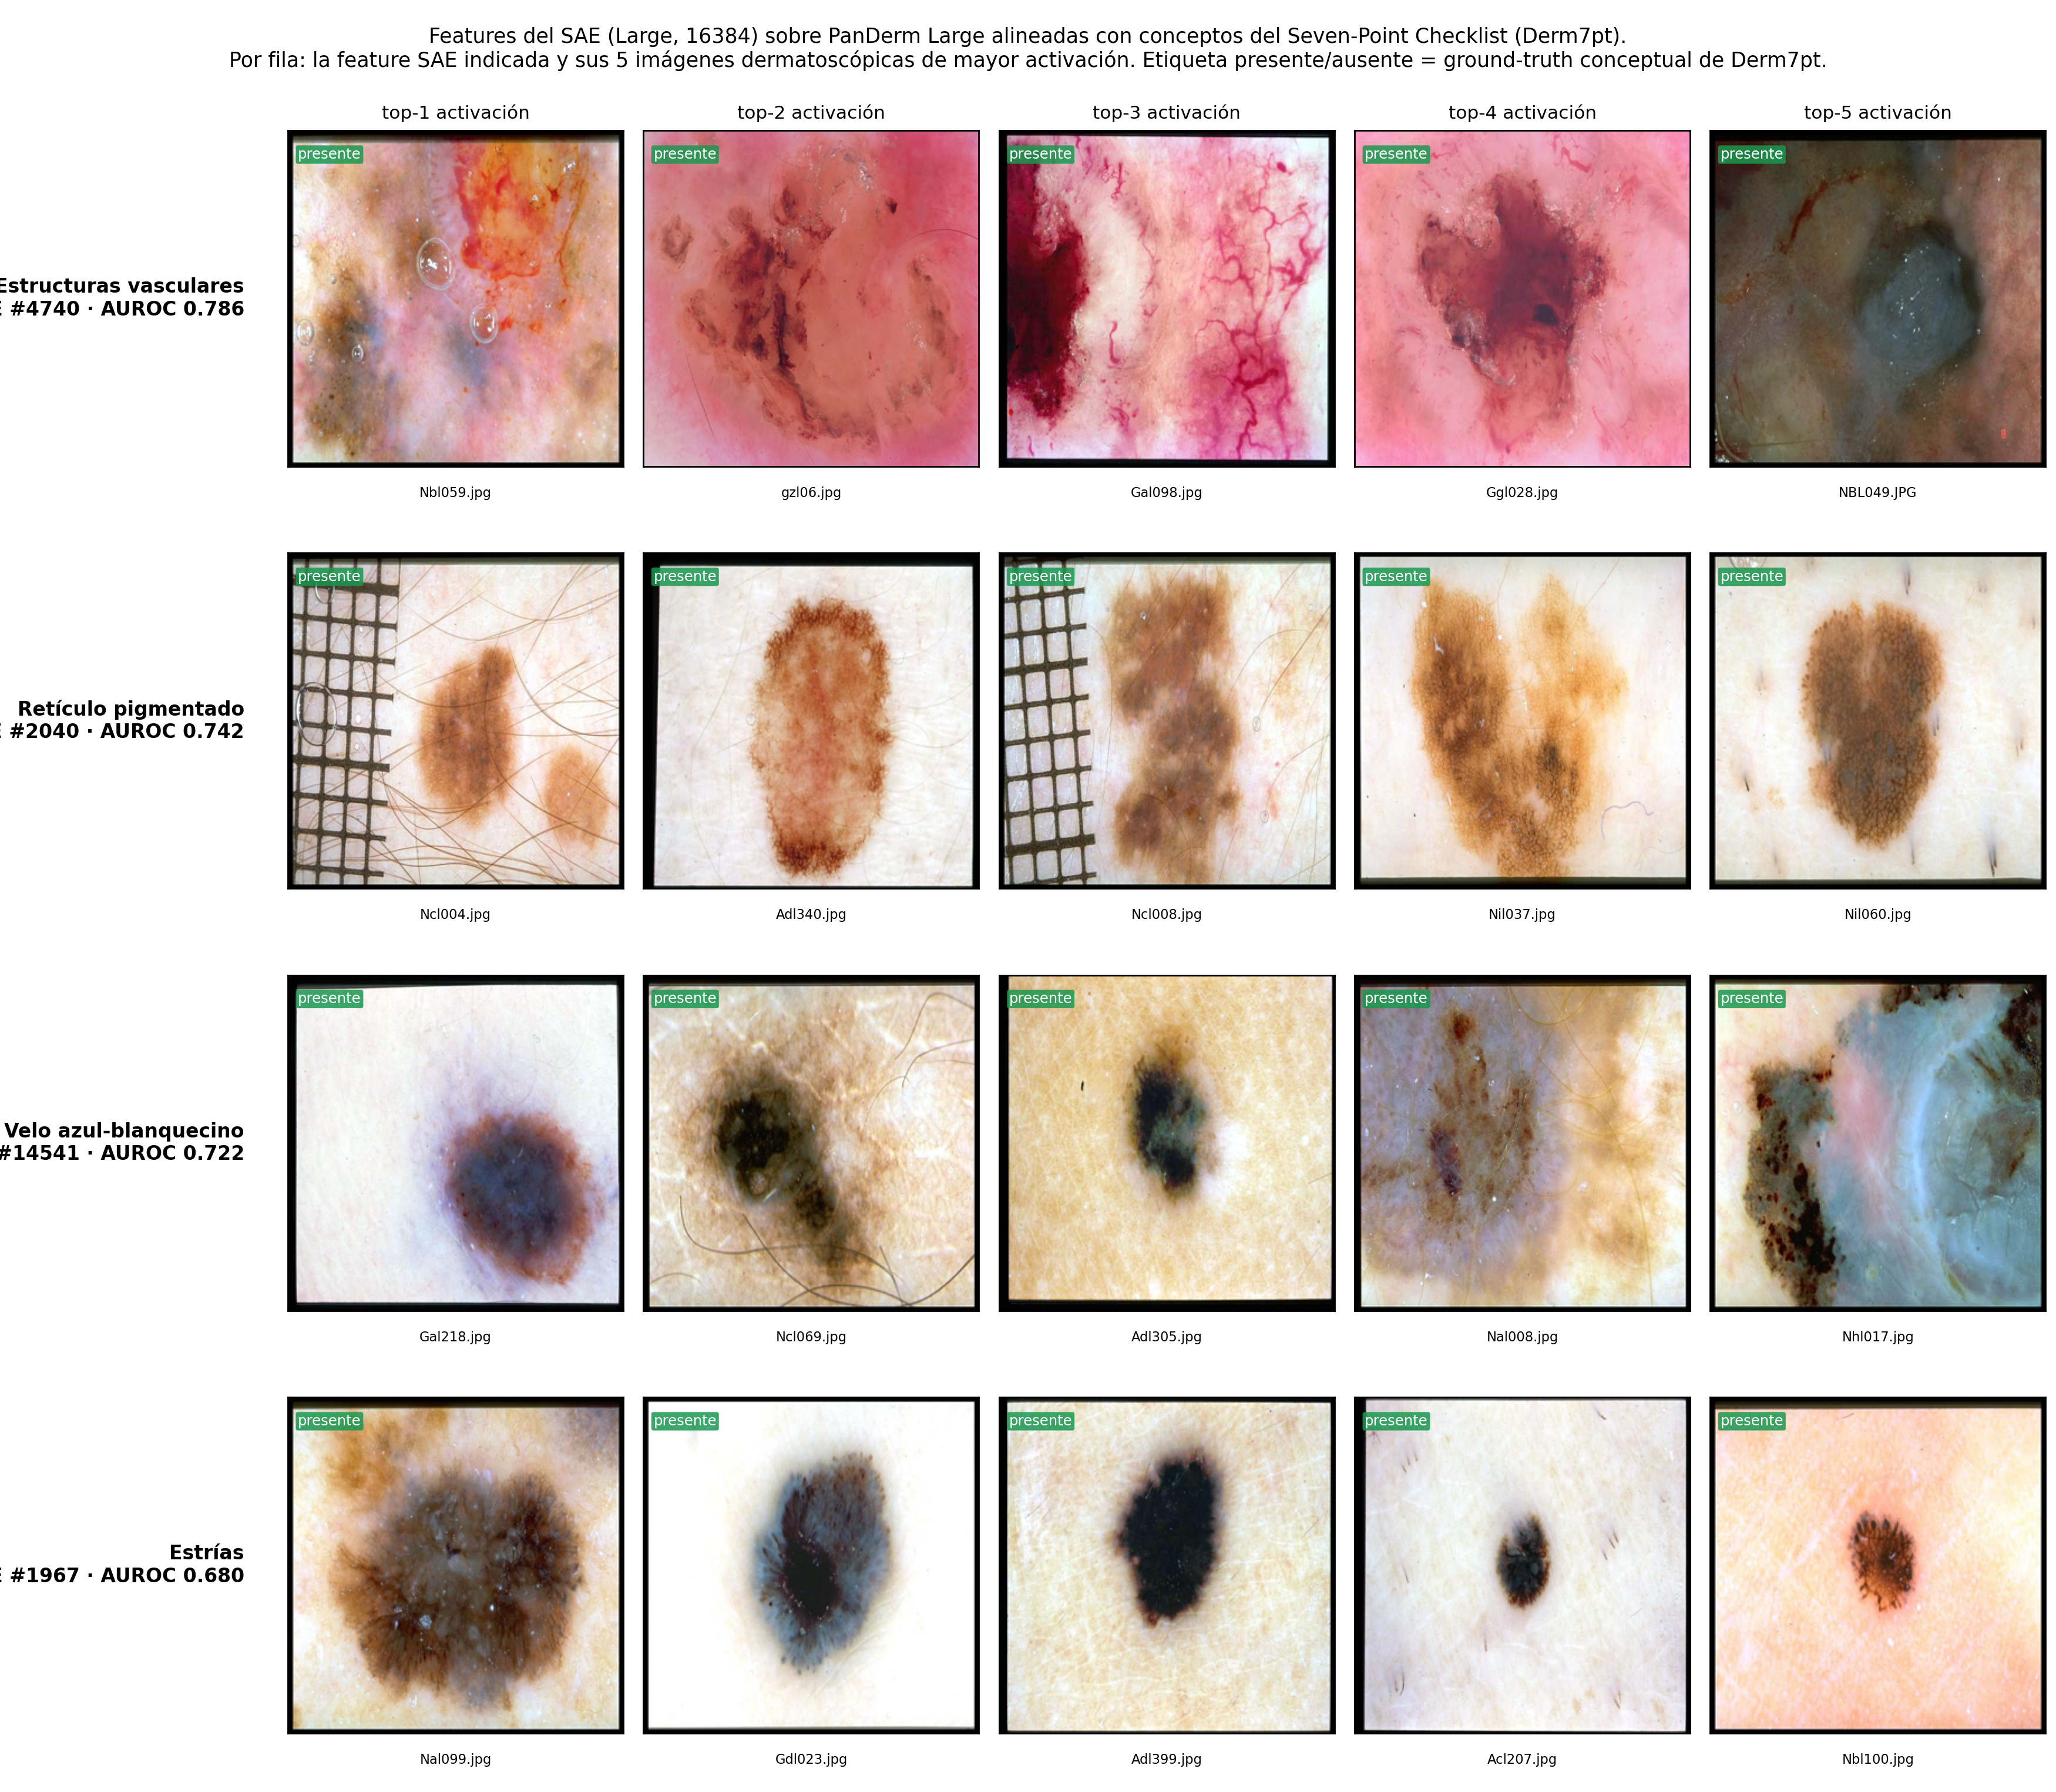
\includegraphics[width=\textwidth]{fig_sae_concepts.png}
\caption{Alineamiento de \emph{features} del SAE con conceptos
dermatoscópicos del \emph{Seven-Point Checklist} (sobre las
$1\,011$ lesiones de Derm7pt). Cada fila es un criterio y una
\emph{feature} del SAE de dirección positiva: las cinco imágenes que más
la activan comparten el concepto clínico (\emph{precision}@5 $= 1{,}0$
en las cuatro). AUROC efectivo de cada \emph{feature}: estructuras
vasculares $0{,}785$ (feat.~4740), retículo pigmentado $0{,}742$
(feat.~2040), velo azul-blanquecino $0{,}722$ (feat.~14541) y estrías
$0{,}680$ (feat.~1967). Se muestra, por criterio, una \emph{feature}
representativa con \emph{top-5} íntegramente concepto-positivo; su AUROC
puede quedar algo por debajo del máximo absoluto del criterio, que
incluye \emph{features} de dirección negativa. Las etiquetas
presente/ausente proceden del \emph{ground-truth} del \emph{Seven-Point
Checklist}.}
\label{fig:sae-concepts}
\end{figure}

\paragraph{¿Y si lo obligamos a decidir solo con esos conceptos?}
El siguiente paso es pasar de ``detectar conceptos'' a ``decidir a
través de ellos''. La forma más transparente es un \emph{Concept
Bottleneck Model}: el modelo primero estima los siete criterios y, solo
a partir de esas siete estimaciones, decide melanoma/no-melanoma. Es
máximamente explicable ---toda la decisión pasa por conceptos con
nombre---, pero cuesta precisión: la AUROC baja de $0{,}890$ a $0{,}832$
($-5{,}8$\,pp). A cambio, hay un detalle tranquilizador: el modelo da
más peso al velo azul-blanquecino y a las estructuras de regresión,
justo los dos criterios que el \emph{Seven-Point
Checklist}~\cite{kawahara2019} puntúa más alto. Las cifras se comparan
en la tabla~\ref{tab:sae-d7pt-e4-comp}.

\paragraph{Hacia un vocabulario propio, en castellano, con la
Dra.~Taberner.}
Hasta aquí los conceptos venían ``prestados'' de escalas en inglés
(SkinCon, \emph{Seven-Point Checklist}). La idea que da sentido a toda
esta línea es construir un vocabulario propio junto a un especialista.
Como primer paso se propusieron $16$ conceptos dermatoscópicos
(Grupo~A) a la Dra.~R.~Taberner: al cruzarlos con el \emph{Seven-Point
Checklist}, $11$ tienen equivalencia directa y $7$ de ellos ya están
capturados por alguna \emph{feature} del SAE con AUROC $\geq 0{,}70$
---incluido uno con apenas $15$ casos positivos, señal de que el SAE
detecta también patrones poco frecuentes---. Los $5$ restantes no
figuran en las escalas clásicas: son precisamente los que justifican ir
más allá.

Para ello se ha desarrollado una plataforma de anotación con la que la
Dra.~Taberner está definiendo un vocabulario dermatoscópico propio y
mucho más amplio: una matriz que asocia alrededor de $35$ estructuras
---retículo pigmentado, velo blanco-azulado, telangiectasias
arboriformes, lagunas rojas, estructuras en hoja de arce, lágrimas
amarillas o el signo del ala delta, entre otras--- con $15$
diagnósticos, indicando qué buscar en cada uno
(figura~\ref{fig:rosa-matrix}). Este vocabulario ampliado todavía no se
ha usado para entrenar ---es trabajo en curso---, pero es la pieza que
permitirá, en el futuro, que las explicaciones del modelo se expresen
en los mismos términos que un dermatólogo emplearía ante el paciente.

\begin{figure}[p]
\centering
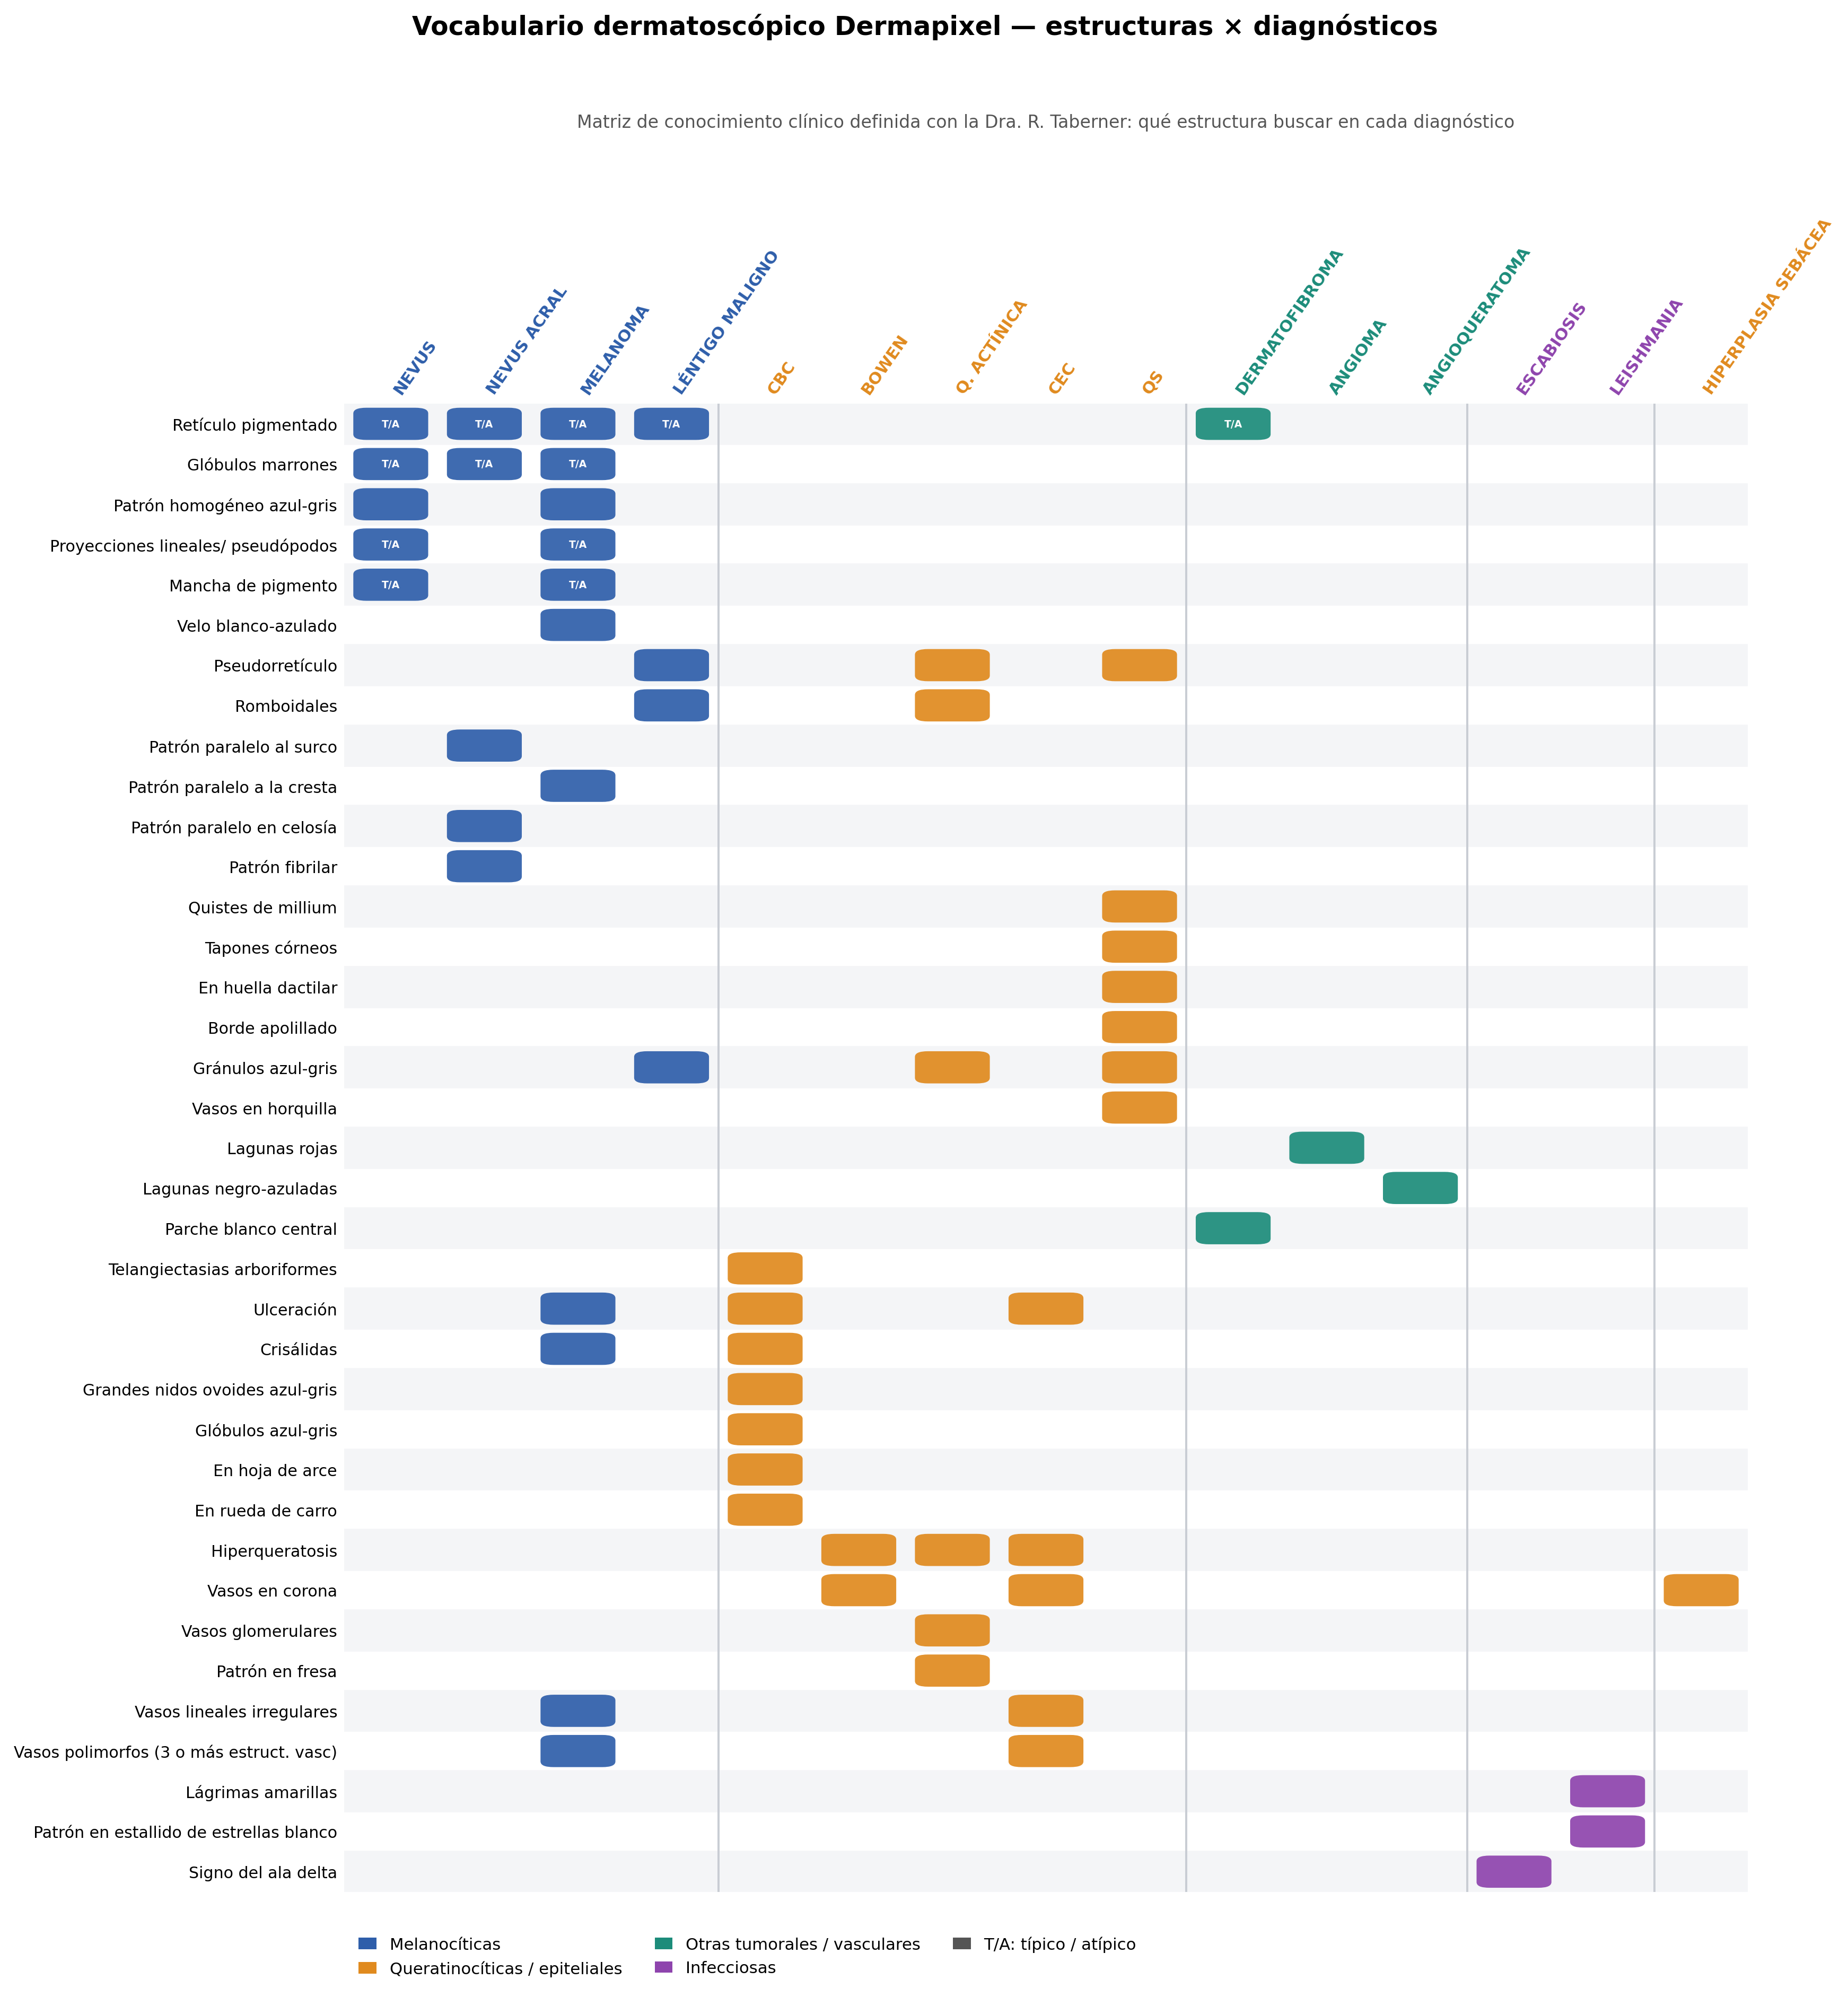
\includegraphics[width=\textwidth]{fig_rosa_matrix.png}
\caption{Vocabulario dermatoscópico que la Dra.~R.~Taberner está
definiendo en la plataforma de anotación: $37$ estructuras
dermatoscópicas (filas) asociadas a $15$ diagnósticos (columnas,
coloreadas por familia: melanocíticas, queratinocíticas o epiteliales,
otras tumorales/vasculares e infecciosas). Cada celda marca qué
estructura buscar en cada diagnóstico; ``T/A'' señala las estructuras
con distinción típico/atípico. Más amplio que las escalas clásicas, es
la base prevista para que, en el futuro, el modelo explique sus
decisiones en castellano (todavía no usado para entrenar).}
\label{fig:rosa-matrix}
\end{figure}

\subsection*{Explicación y rendimiento a la vez}
\label{sec:sae-d7pt-e4}

La pregunta final es si se puede tener lo mejor de los dos mundos:
explicación \emph{y} precisión. La respuesta es que sí. En lugar del
cuello de botella estricto del apartado anterior, se entrena el modelo
para predecir a la vez el melanoma y los siete conceptos ---ocho
\emph{heads} (salidas) en paralelo, siguiendo el esquema multitarea de
Kawahara et~al.~\cite{kawahara2019}--- con una adaptación ligera: LoRA
($r = 16$) sobre los dos últimos bloques de PanDerm Large, el mismo
esquema que Dermapixel R0 (sección~\ref{sec:dermapixel-spanderm-v0}),
con solo $0{,}56$\,M parámetros entrenables ($0{,}18\%$ del modelo).
Sobre el test de Derm7pt ($N_{\mathrm{test}} = 395$), el resultado
(tabla~\ref{tab:sae-d7pt-e4-comp}) es el mejor posible: la salida de
melanoma alcanza una AUROC de $0{,}891$ ---idéntica a la del modelo sin
ninguna restricción ($0{,}890$) y $5{,}9$\,pp por encima del
\emph{Concept Bottleneck}--- y, además, entrega los siete conceptos en
la misma pasada, sin coste apreciable.

\begin{table}[htbp]
\centering
\footnotesize
\setlength{\tabcolsep}{4pt}
\renewcommand{\arraystretch}{0.95}
\caption{Comparativa sobre la tarea binaria melanoma/no-melanoma
entre el linear probe directo sobre las $16\,384$ \emph{features}
del SAE Large, el \emph{Concept Bottleneck} de siete conceptos y el
fine-tuning multitarea LoRA con ocho \emph{heads} paralelas. Conjunto
de test Derm7pt ($N_{\mathrm{test}} = 395$, $n_{\mathrm{mel}} \approx
98$), mismo \emph{split} oficial. AUROC en negrita.}
\label{tab:sae-d7pt-e4-comp}
\begin{tabular}{lrrrrrr}
\hline
Método                                       & Params entr. & Acc@1     & BAcc      & AUROC              & W-F1      & Kappa     \\
\hline
Linear probe directo (SAE $\to$ mel)          & $16$\,K       & $0{,}841$ & $0{,}735$ & $0{,}890$          & $0{,}829$ & $0{,}527$ \\
Concept Bottleneck (SAE $\to$ $7$ conc.\ $\to$ mel) & $\sim 120$ & $0{,}825$ & $0{,}681$ & $0{,}832$          & $0{,}801$ & $0{,}440$ \\
\textbf{Multitarea LoRA ($8$ salidas)}        & $0{,}56$\,M   & $\mathbf{0{,}841}$ & $\mathbf{0{,}804}$ & $\mathbf{0{,}891}$ & $\mathbf{0{,}843}$ & $\mathbf{0{,}590}$ \\
\hline
\end{tabular}
\end{table}

En conjunto, esta línea deja tres mensajes. Primero, que las
representaciones de PanDerm ya están organizadas en torno a conceptos
clínicos, sin habérselo pedido. Segundo, que sobre ellas se puede
construir un sistema que explica sus decisiones en el lenguaje del
dermatólogo sin sacrificar precisión, siempre que los conceptos encajen
con la tarea ---como ocurre con el \emph{Seven-Point
Checklist}~\cite{kawahara2019}---. Y tercero, que el paso siguiente
---un vocabulario dermatoscópico propio, definido con la
Dra.~Taberner--- ya está en marcha. Es la base sobre la que se apoya el
módulo de explicabilidad del prototipo (repositorio reproducible,
\ref{cap:repo}, sección~\ref{sec:repo-prototipo}).
